\documentclass[11pt, a4paper]{article}

% --- UNIVERSAL PREAMBLE BLOCK ---
\usepackage[a4paper, top=2.5cm, bottom=2.5cm, left=2cm, right=2cm]{geometry}
\usepackage{fontspec}
\usepackage{graphicx}
\usepackage{xcolor}

\usepackage[english]{babel}

% Set default/Latin font to Sans Serif in the main slot
\setmainfont{DejaVu Sans}

% Packages for flowchart, graphics, and plots
\usepackage{tikz}
\usetikzlibrary{shapes.geometric, arrows.meta, positioning, fit, backgrounds, calc, shadows, patterns}
\usepackage{pgfplots}
\pgfplotsset{compat=1.18}
\usepackage{caption}

% Packages for formatting and structure
\usepackage{enumitem}
\usepackage{booktabs}
\usepackage{amsmath}
\usepackage{titlesec}
\usepackage{setspace}
\usepackage{float}

% Absorb minor line-breaking overflows with the sans-serif body font
\emergencystretch=2.5em
\hbadness=10000

% Number figures and tables per section (e.g. Figure 2.1, Table 3.2)
\numberwithin{figure}{section}
\numberwithin{table}{section}

% Title Formatting
\titleformat{\section}{\Large\bfseries}{\thesection}{1em}{}
\titleformat{\subsection}{\large\bfseries}{\thesubsection}{1em}{}

% ============================================================
% PRINT-SAFE MONOCHROME SCHEME
% All figures use a greyscale ramp with clearly separated
% luminance steps, reinforced by distinct hatch patterns, so
% that every series remains distinguishable when the report is
% printed or photocopied in black and white.
% ============================================================
\definecolor{alPrimary}{gray}{0.25}
\definecolor{alSecondary}{gray}{0.55}
\definecolor{alAccent}{gray}{0.80}
\definecolor{alDeep}{gray}{0.10}
\definecolor{alGrey}{gray}{0.68}

% Greyscale ramp for multi-series charts (light -> dark)
\definecolor{g1}{gray}{0.95}
\definecolor{g2}{gray}{0.86}
\definecolor{g3}{gray}{0.76}
\definecolor{g4}{gray}{0.66}
\definecolor{g5}{gray}{0.56}
\definecolor{g6}{gray}{0.46}
\definecolor{g7}{gray}{0.36}
\definecolor{g8}{gray}{0.26}
\definecolor{g9}{gray}{0.14}

% Country fills for the exporter chart: greyscale ramp, each
% reinforced with its own hatch pattern (defined at point of use)
\definecolor{cMalaysia}{gray}{0.20}
\definecolor{cUAE}{gray}{0.92}
\definecolor{cBahrain}{gray}{0.55}
\definecolor{cQatar}{gray}{0.78}
\definecolor{cRussia}{gray}{0.36}
\definecolor{cKorea}{gray}{0.66}
\definecolor{cOman}{gray}{0.10}
\definecolor{cVietnam}{gray}{0.86}
\definecolor{cSaudi}{gray}{0.46}
\definecolor{cThailand}{gray}{0.72}
\definecolor{cIndonesia}{gray}{0.60}
\definecolor{cSouthAfrica}{gray}{0.30}

\definecolor{exMalaysia}{gray}{0.20}
\definecolor{exUAE}{gray}{0.92}
\definecolor{exBahrain}{gray}{0.55}
\definecolor{exQatar}{gray}{0.78}
\definecolor{exRussia}{gray}{0.36}
\definecolor{exKorea}{gray}{0.66}
\definecolor{exOman}{gray}{0.10}
\definecolor{exVietnam}{gray}{0.86}
\definecolor{exSaudi}{gray}{0.46}
\definecolor{exThailand}{gray}{0.72}
\definecolor{exIndonesia}{gray}{0.60}
\definecolor{exSouthAfrica}{gray}{0.30}

% ---------------------------------------------------------

\title{\textbf{Rationalizing Tariff Structures in the Indian Downstream Aluminium Industry}\\
\Large Addressing the Inverted Duty Structure to Maximize Value Addition and Employment}
\author{}
\date{}

\begin{document}

\maketitle

\begin{abstract}
    \noindent \textit{Executive Summary: This report highlights the urgent need to rationalize the tariff regime governing downstream aluminium input products (HS 7601--7616). Currently, the sector suffers from an Inverted Duty Structure (IDS) driven by Preferential Trade Agreements (PTAs), which severely depresses the Effective Rate of Protection (ERP) for domestic manufacturers. Synthesizing empirical data for the fiscal year 2021-22, we demonstrate that this structure penalizes domestic industrial players—stifling Gross Value Added (GVA) and job creation in this labour-intensive segment—and creates a "lose-lose" scenario for Indian consumers through compromised supply chain resilience and limited product variety. Beyond the tariff wedge itself, the report shows how geopolitical chokepoints, subsidised Chinese competition, and emerging carbon-compliance regimes compound the disadvantage faced by domestic Micro, Small, and Medium Enterprises (MSMEs). Correcting these anomalies is a strategic economic imperative to support domestic MSMEs and unlock national employment opportunities.}
\end{abstract}

\vspace{1cm}
\tableofcontents
\newpage

\section{Introduction}

\subsection{Aluminium as a Strategic Metal}
Aluminium is the third most abundant element in the Earth's crust---accounting for roughly 8\%---and the single most abundant metal, though its reactive nature means it occurs in nature only in bound alumino-silicate forms rather than as free metal \cite{mom_vision2025}\footnote{Ministry of Mines, Government of India. (2025). \textit{Vision Document on Aluminium Metal for India}.}. Over the past six decades global aluminium consumption has grown more than twenty-fold, one of the fastest expansions of any industrial metal. A distinctive combination of properties---light weight, high electrical and thermal conductivity, corrosion resistance, formability, and near-infinite recyclability---has made it the second-most consumed metal in the world after steel, with global consumption of approximately 97.8 million tonnes in 2023 \cite{mom_vision2025}\footnote{Ministry of Mines, \textit{Vision Document on Aluminium Metal for India} (2025).}. Having overtaken copper in 1954 to become the most-produced non-ferrous metal, aluminium today accounts for more output than all other non-ferrous metals combined---some 108 MT in 2022, against roughly 26 MT for copper.

Often described as the ``metal of the future,'' aluminium underpins a remarkably broad set of end-uses: automobiles and surface transport, building and construction, packaging, electrical transmission, machinery and equipment, aerospace and defence, and consumer durables \cite{mom_vision2025}\footnote{Ministry of Mines, \textit{Vision Document on Aluminium Metal for India} (2025).}. Its low weight and recyclability place it at the centre of the global low-carbon transition---as a lightweighting material for electric vehicles, a structural input for renewable-energy infrastructure, and an enabler of energy-efficient buildings---while its infinite recyclability aligns naturally with circular-economy principles. These attributes have led governments worldwide to treat aluminium as a strategic industry: China formally designates it a ``pillar industry,'' the United States classifies it among the minerals critical to national defence and energy security, and the European Union, Russia, Canada, South Korea and the Gulf economies have each built dedicated industrial strategies around the metal.

\subsection{Strategic Importance for the Indian Economy}
For India, the strategic significance of aluminium spans economic growth, infrastructure development, defence, transportation, sustainability, and global competitiveness. As of the financial year 2024, India's installed primary aluminium capacity stood at 4.17 million tonnes, making it the second-largest primary producer in the world. Yet India's per capita consumption remains remarkably low---roughly 3.5 kg (FY24) against a global average of about 12 kg, and only a fraction of the levels seen in mature markets such as South Korea (42.8 kg, the world's highest), Bahrain (32 kg) and Germany (31 kg) \cite{mom_vision2025}\footnote{Ministry of Mines, \textit{Vision Document on Aluminium Metal for India} (2025).}. This gap signals an enormous, largely untapped domestic growth runway. Propelled by rapid urbanization, electrification of the grid, and the transition to electric mobility, domestic demand is projected to surge to 8.5 MT by FY30 and 28 MT by FY47 \cite{mom_vision2025}\footnote{Ministry of Mines, \textit{Vision Document on Aluminium Metal for India} (2025).}.

These aggregate projections translate into an exceptional, and specifically downstream, opportunity. The bulk of India's incremental demand to FY47 is expected to arise not from primary metal but from higher-intensity and new-to-India value-added applications---an estimated 15--18 MT from deeper penetration of existing uses (defence and civil-aviation airframes, packaged food and beverage, and the like) and a further 4--6 MT from newer applications such as greater aluminium content in automobiles and transport---precisely the product categories fabricated by downstream MSMEs \cite{mom_vision2025}\footnote{Ministry of Mines, \textit{Vision Document on Aluminium Metal for India} (2025).}. On the trade side, India today remains a fringe player in the roughly 67 MT global aluminium market, holding a share of just 3.8\% against China's 12.6\%; national strategy targets lifting this to about 10\% by FY47 while deliberately reorienting the export mix towards value-added downstream products rather than raw metal, and maximising the conversion of primary output into downstream goods by 2035 \cite{mom_vision2025}\footnote{Ministry of Mines, \textit{Vision Document on Aluminium Metal for India} (2025).}. Set against India's broader ambition of becoming a US\$30 trillion economy, capturing even a fraction of this trajectory would require the downstream sector to expand several-fold---underscoring why the structural disadvantages it currently faces carry consequences far beyond the firms directly affected.

Whether any of this potential is realised depends, above all, on the downstream sector. Comprising over 3,500 Micro, Small, and Medium Enterprises (MSMEs), it is the primary engine of value addition, employment, and product innovation in the aluminium economy---and, as this report argues, the segment most exposed to the structural tariff anomalies examined in the sections that follow. 

Two things about this downstream segment explain why it is so sensitive to policy. The first is that, unlike the highly consolidated and capital-intensive upstream smelting industry, downstream fabrication is geographically dispersed, fragmented, and dominated by small firms operating on structurally thin margins, leaving it far more exposed to external cost shocks \cite{costreg2026}\footnote{\textit{Comprehensive Economic Analysis of the Global Downstream Aluminium Industry}, 2026 (synthesis of trade data and peer-reviewed literature). \cite{costreg2026}.}. The second is that the price of its main raw material is not set at home at all. It is tethered to a global benchmark that is itself highly volatile: empirical analysis of non-ferrous metals finds strong---and, since the financialisation of commodity markets, intensifying---spillovers from geopolitical risk and global economic-policy uncertainty into aluminium prices \cite{bensalha2025}\footnote{Ben-Salha, O., Zmami, M., Waked, S.~S., Najjar, F., \& Alenazi, Y.~M. (2025). \textit{On the time-varying spillover between nonferrous metals prices, geopolitical risks, and global economic policy uncertainty.} Economic Change and Restructuring, 58(5). \cite{bensalha2025}.}. So the segment that adds the most value and creates the most jobs is also the one least sheltered from forces well outside its control. Tariff design has, so far, largely ignored that asymmetry. 

Nothing throws this asymmetry into sharper relief than the contrasting financial health of the two segments. India's consolidated primary producers are not fragile entrants in need of tariff protection but highly profitable incumbents. Brokerage analysis of the country's fastest-expanding primary producer, for instance, projects operating earnings (EBITDA) compounding at roughly 29\% a year over FY26--FY28 to around INR 419 billion (about US\$4.4 billion), even as its hot-metal cost of production falls from approximately US\$1,914 per tonne to below US\$1,600 and its net debt is all but extinguished \cite{alcircle2026}\footnote{``Vedanta Aluminium to rally 22\%? Nuvama initiates `Buy' with 29\% EBITDA forecast,'' \textit{AL Circle}, 14 July 2026.}. Set against operating surpluses of that size, the 7.5\% basic customs duty on primary metal protects producers who are already thriving---which is to say, it protects very little. What it does in practice is transfer margin from a thin-margin downstream sector to a comfortably profitable upstream one. Raising input duties further would therefore shield nothing that genuinely requires shielding, whereas rationalising them downward would pass through directly to the competitiveness---and, for many firms, the survival---of the downstream fabricators on which the sector's value addition and employment depend.

\subsection{Scope and Objective: Focus on HS Codes 7601--7616}
The objective of this report is to advocate for the rationalization of tariff lines for input products utilized in the downstream aluminium categories (HS Codes 7601--7616). We argue that the current tariff structure disproportionately harms domestic players and must be realigned to support domestic manufacturing and value chain integration. This is not a novel position; it rests on a body of existing scholarship. India-focused research has argued that lowering import duties on primary aluminium---particularly low-carbon metal from producers such as Canada, Norway and Iceland---would normalise domestic input prices and directly raise the competitiveness of the downstream sector, including its capacity to export value-added products to carbon-regulated markets \cite{arora2023}\footnote{Arora, A. (2023). \textit{Assessing the Impact of CBAM and Tariffs in the Indian Aluminum Industry.} IIFT Working Paper Series, WPS No.~EC-23-65, Indian Institute of Foreign Trade, New Delhi. \cite{arora2023}.}. More broadly, the trade-and-development literature establishes that access to competitively priced and varied intermediate inputs is a principal driver of domestic product growth and innovation---evidence drawn, notably, from India's own experience with input-tariff liberalisation \cite{goldberg2010}\footnote{Goldberg, Khandelwal, Pavcnik \& Topalova (2010), \textit{Imported Intermediate Inputs and Domestic Product Growth}. \cite{goldberg2010}.}.

\subsection{The Aluminium Value Chain}
As illustrated in Figure \ref{fig:value_chain} (reproduced in Appendix~B), the aluminium manufacturing process involves three distinct phases, spanning from raw extraction to advanced fabrication.

\begin{itemize}
    \item \textbf{Phase 1 (Upstream):} The cycle begins with the mining of bauxite ore, which is refined into alumina and subsequently smelted into unwrought primary aluminium (HS 7601). Recycled scrap (HS 7602) also enters the metallurgical cycle at this stage.
    \item \textbf{Phase 2 (Midstream / Downstream Genesis):} This unwrought metal is cast, extruded, rolled, or drawn into essential semi-finished goods such as bars, plates, sheets, foils, and wire (HS 7604--7609).
    \item \textbf{Phase 3 (Downstream):} These intermediate inputs are transformed into specialized, highly value-added end products, including architectural structures, packaging containers, household utensils, and electrical cables (HS 7610--7616).
\end{itemize}
This report specifically addresses the structural trade imbalances occurring as materials move from Phase 1 into Phases 2 and 3.

\begin{figure}[H]
    \centering
    \resizebox{\textwidth}{!}{%
    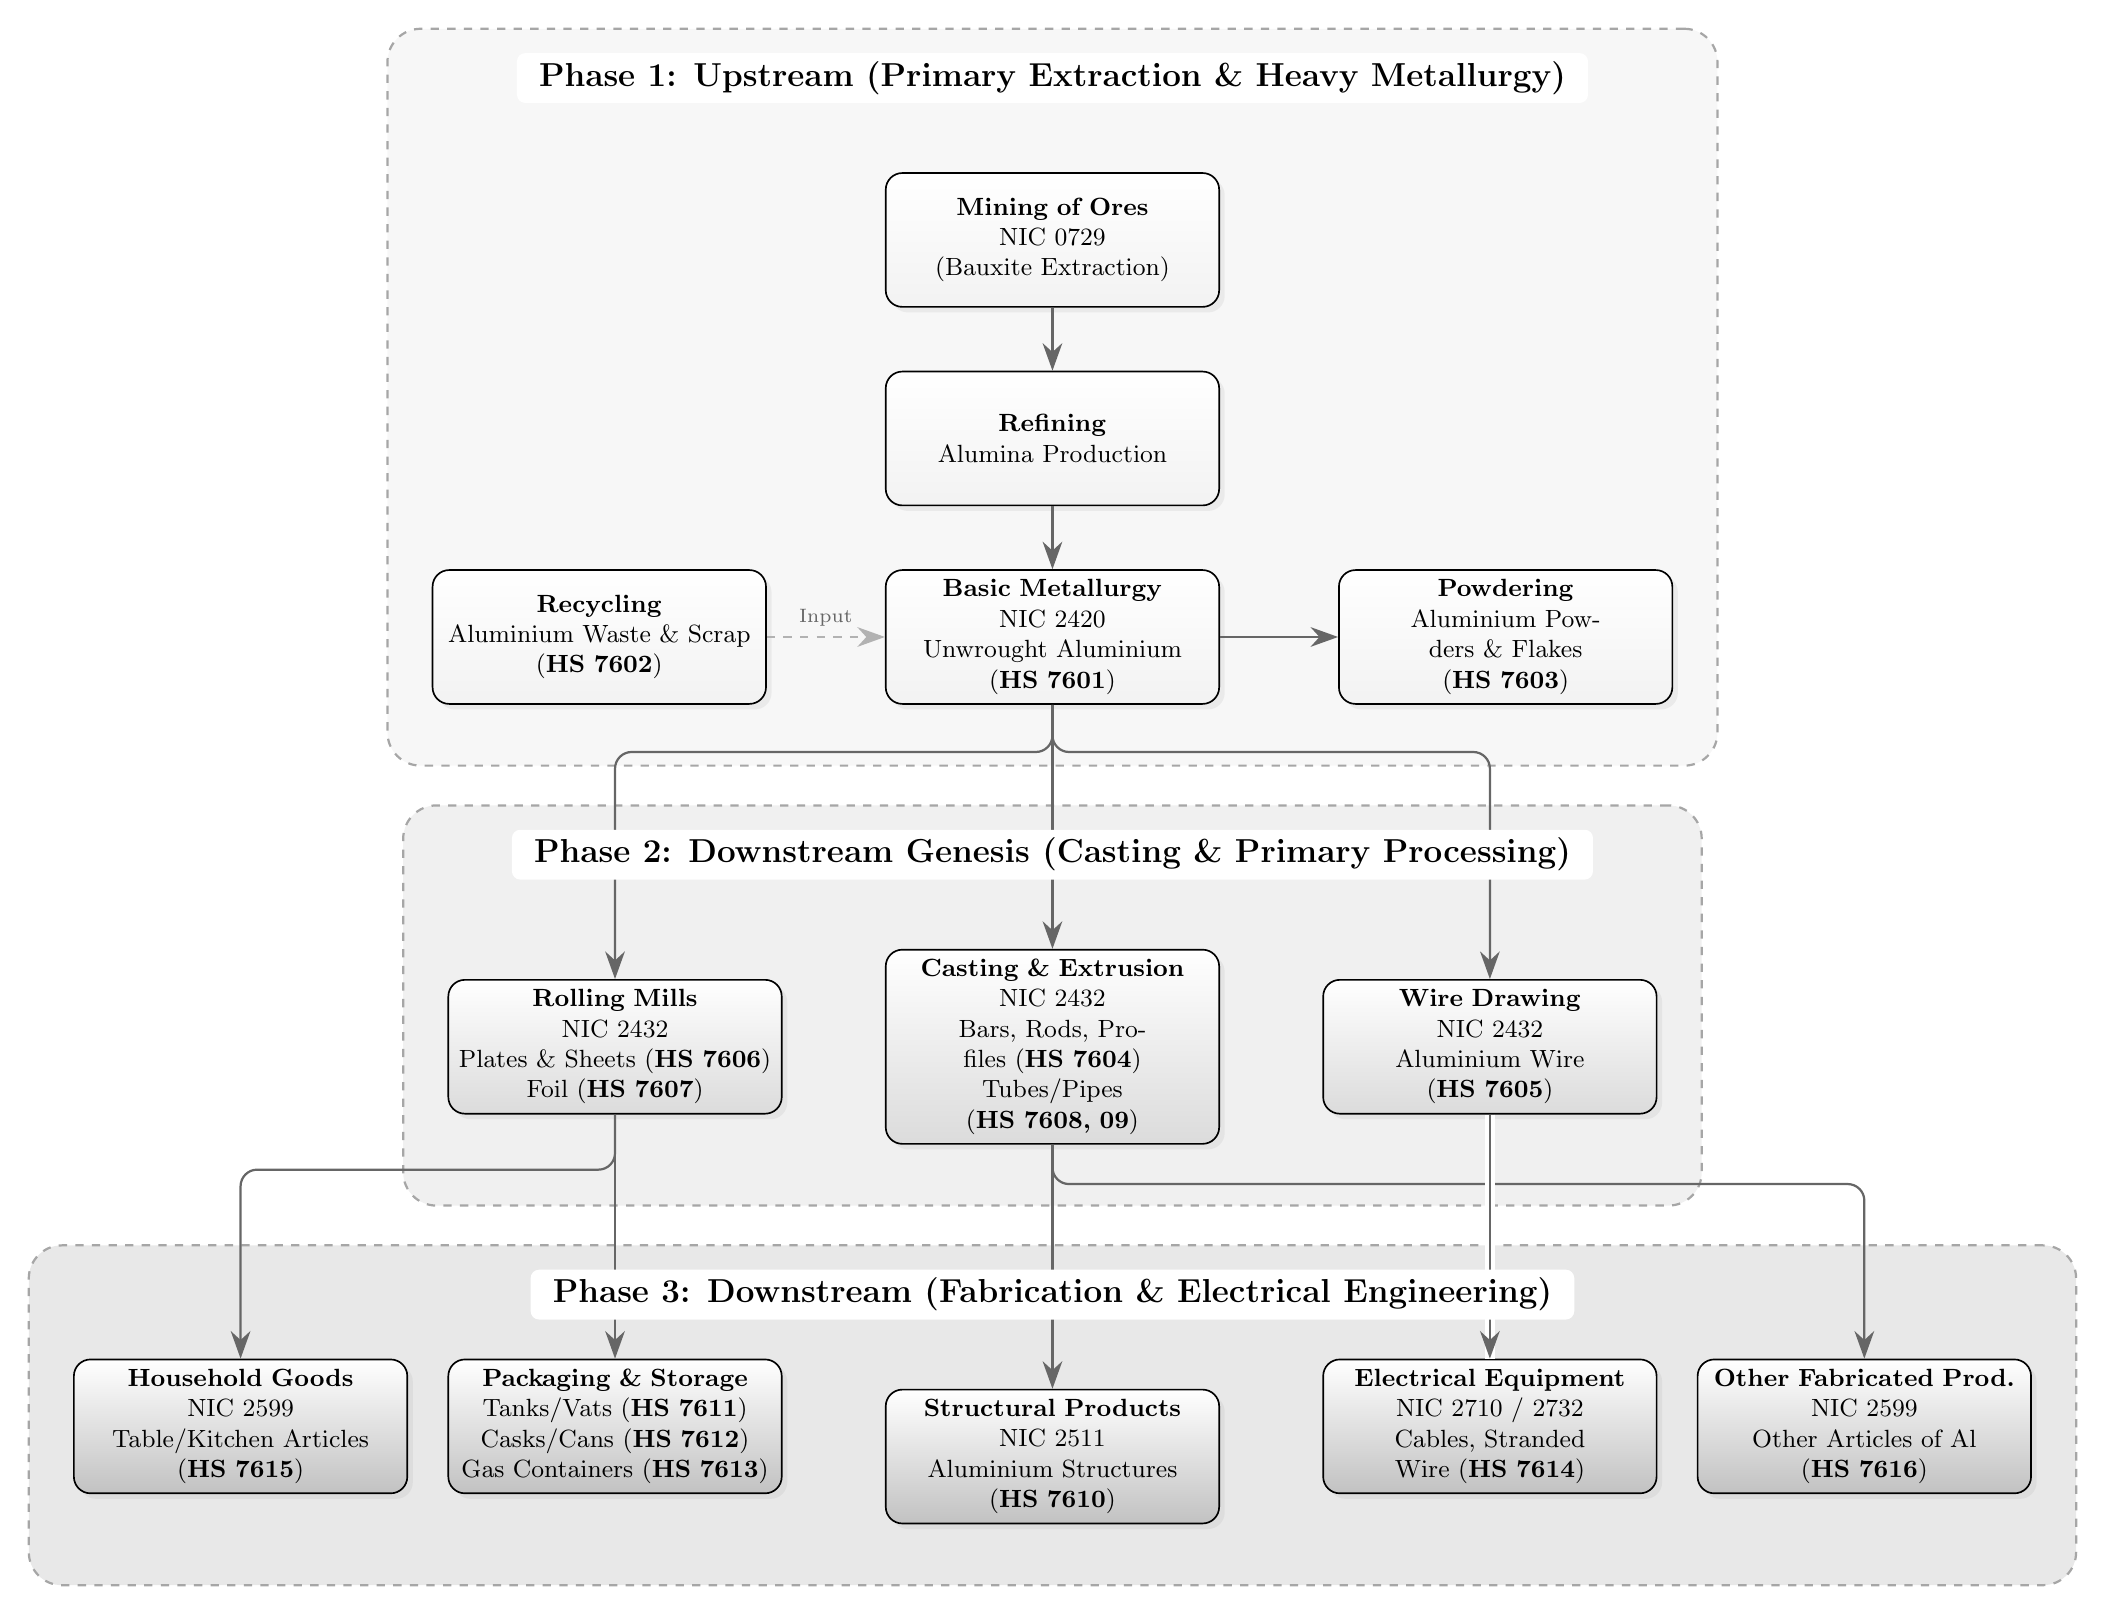
\begin{tikzpicture}[
        node distance=1.5cm and 1.3cm,
        box/.style={rectangle, draw, rounded corners=6pt, align=center, text width=4.0cm, minimum height=1.7cm, thick, font=\small, drop shadow={opacity=0.1, shadow xshift=2pt, shadow yshift=-2pt}},
        up/.style={box, top color=white, bottom color=g1, draw=black, line width=0.6pt},
        mid/.style={box, top color=white, bottom color=g2, draw=black, line width=0.6pt},
        down/.style={box, top color=white, bottom color=g3, draw=black, line width=0.6pt},
        arrow/.style={-{Stealth[length=3.5mm, width=2.5mm]}, thick, draw=gray!80!black, rounded corners=6pt},
        backarrow/.style={dashed, -{Stealth[length=3.5mm, width=2.5mm]}, thick, draw=gray!60, rounded corners=6pt},
        groupbox/.style={rectangle, rounded corners=12pt, draw=black!35, dashed, thick, inner xsep=16pt, inner ysep=22pt}
    ]
        % UPSTREAM PHASE
        \node[up] (unwrought) {\textbf{Basic Metallurgy} \\ NIC 2420 \\ Unwrought Aluminium \\ (\textbf{HS 7601})};
        \node[up] (alumina) [above=0.8cm of unwrought] {\textbf{Refining} \\ Alumina Production};
        \node[up] (bauxite) [above=0.8cm of alumina] {\textbf{Mining of Ores} \\ NIC 0729 \\ (Bauxite Extraction)};
        \node[up] (scrap) [left=1.5cm of unwrought] {\textbf{Recycling} \\ Aluminium Waste \& Scrap \\ (\textbf{HS 7602})};
        \node[up] (powder) [right=1.5cm of unwrought] {\textbf{Powdering} \\ Aluminium Powders \& Flakes \\ (\textbf{HS 7603})};

        % MIDSTREAM PHASE
        \node[mid] (extrusion) [below=3.1cm of unwrought] {\textbf{Casting \& Extrusion} \\ NIC 2432 \\ Bars, Rods, Profiles (\textbf{HS 7604}) \\ Tubes/Pipes (\textbf{HS 7608, 09})};
        \node[mid] (rolling) [left=1.3cm of extrusion] {\textbf{Rolling Mills} \\ NIC 2432 \\ Plates \& Sheets (\textbf{HS 7606}) \\ Foil (\textbf{HS 7607})};
        \node[mid] (drawing) [right=1.3cm of extrusion] {\textbf{Wire Drawing} \\ NIC 2432 \\ Aluminium Wire \\ (\textbf{HS 7605})};

        % DOWNSTREAM PHASE
        \node[down] (structures) [below=3.1cm of extrusion] {\textbf{Structural Products} \\ NIC 2511 \\ Aluminium Structures \\ (\textbf{HS 7610})};
        \node[down] (containers) [below=3.1cm of rolling] {\textbf{Packaging \& Storage} \\ Tanks/Vats (\textbf{HS 7611}) \\ Casks/Cans (\textbf{HS 7612}) \\ Gas Containers (\textbf{HS 7613})};
        \node[down] (household) [left=0.5cm of containers] {\textbf{Household Goods} \\ NIC 2599 \\ Table/Kitchen Articles \\ (\textbf{HS 7615})};
        \node[down] (cables) [below=3.1cm of drawing] {\textbf{Electrical Equipment} \\ NIC 2710 / 2732 \\ Cables, Stranded Wire (\textbf{HS 7614})};
        \node[down] (other) [right=0.5cm of cables] {\textbf{Other Fabricated Prod.} \\ NIC 2599 \\ Other Articles of Al \\ (\textbf{HS 7616})};

        % BACKGROUND GROUPING & LABELS
        \node (up_dummy) [above=0.8cm of bauxite] {};
        \node (mid_dummy) [above=0.8cm of extrusion] {};
        \node (down_dummy) [above=0.8cm of structures] {};
        \begin{scope}[on background layer]
            \node[groupbox, fill=black!3, fit=(up_dummy) (bauxite) (alumina) (unwrought) (scrap) (powder)] (up_group) {};
            \node[groupbox, fill=black!6, fit=(mid_dummy) (rolling) (extrusion) (drawing)] (mid_group) {};
            \node[groupbox, fill=black!9, fit=(down_dummy) (household) (containers) (structures) (cables) (other)] (down_group) {};
        \end{scope}


        % ARROWS
        \draw[arrow] (bauxite) -- (alumina);
        \draw[arrow] (alumina) -- (unwrought);
        \draw[backarrow] (scrap) -- node[above, font=\scriptsize, color=gray!80!black] {Input} (unwrought);
        \draw[arrow] (unwrought) -- (powder);
        \draw[arrow] (unwrought.south) -- +(0,-0.6) -| (rolling.north);
        \draw[arrow] (unwrought.south) -- (extrusion.north);
        \draw[arrow] (unwrought.south) -- +(0,-0.6) -| (drawing.north);
        \draw[arrow] (rolling.south) -- (containers.north);
        \draw[arrow] (rolling.south) -- +(0,-0.7) -| (household.north);
        \draw[arrow] (extrusion.south) -- (structures.north);
        \draw[arrow] (extrusion.south) -- +(0,-0.5) -| (other.north);
        \draw[line width=3.5pt, white] (drawing.south) -- (cables.north);
        \draw[arrow] (drawing.south) -- (cables.north);

        % PHASE LABELS -- drawn last, with opaque fills, so no connector
        % line can run through the heading text
        \node[anchor=north, font=\large\bfseries, color=black, yshift=-9pt,
              fill=white, rounded corners=3pt, inner xsep=8pt, inner ysep=3pt]
              at (up_group.north) {Phase 1: Upstream (Primary Extraction \& Heavy Metallurgy)};
        \node[anchor=north, font=\large\bfseries, color=black, yshift=-9pt,
              fill=white, rounded corners=3pt, inner xsep=8pt, inner ysep=3pt]
              at (mid_group.north) {Phase 2: Downstream Genesis (Casting \& Primary Processing)};
        \node[anchor=north, font=\large\bfseries, color=black, yshift=-9pt,
              fill=white, rounded corners=3pt, inner xsep=8pt, inner ysep=3pt]
              at (down_group.north) {Phase 3: Downstream (Fabrication \& Electrical Engineering)};
    \end{tikzpicture}
    }
    \captionsetup{font=normalsize, justification=centering}
    \caption{The Aluminium Value Chain, tracking industrial operations and HS Code progression.}
    \label{fig:value_chain}
\end{figure}

\section{International Trade Dynamics}

The global aluminium landscape is characterized by steadily increasing consumption and shifting trade balances. Global primary aluminum consumption has grown consistently over the past decade, and this upward trajectory is reliably forecast to continue through 2029 (see Figure \ref{fig:global_consumption})\footnote{Source: Statista.}.

\begin{figure}[H]
    \centering
    \captionsetup{font={color=black, normalsize}, justification=centering}
    \caption{Global Primary Aluminum Consumption and its Forecast (in million metric tons)}
    \label{fig:global_consumption}
    \vspace{0.5cm}

    \resizebox{\textwidth}{!}{%
    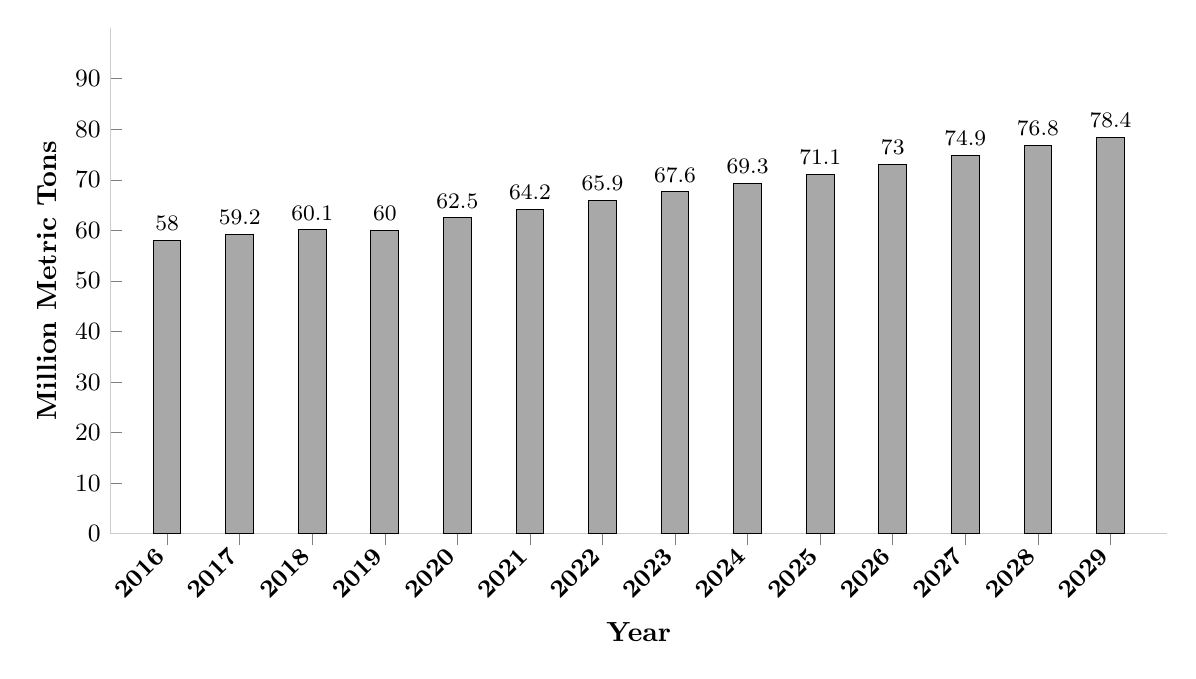
\begin{tikzpicture}
        \begin{axis}[
            ybar,
            width=15cm,
            height=8cm,
            bar width=10pt,
            ymin=0,
            ymax=100,
            ytick={0, 10, 20, 30, 40, 50, 60, 70, 80, 90},
            ylabel={\textbf{Million Metric Tons}},
            xlabel={\textbf{Year}},
            symbolic x coords={2016,2017,2018,2019,2020,2021,2022,2023,2024,2025,2026,2027,2028,2029},
            xtick=data,
            x tick label style={rotate=45, anchor=east, font=\small\bfseries},
            nodes near coords={\textbf{\pgfmathprintnumber\pgfplotspointmeta}},
            nodes near coords align={vertical},
            every node near coord/.append style={font=\footnotesize, color=black},
            tick label style={font=\small\bfseries},
            axis x line*=bottom,
            axis y line*=left,
            enlarge x limits=0.06,
            ymajorgrids=false,
            axis line style={gray!40},
            every axis plot post/.append style={fill=g4, draw=black, line width=0.35pt}
        ]
        \addplot coordinates {
            (2016, 58)
            (2017, 59.2)
            (2018, 60.1)
            (2019, 60)
            (2020, 62.5)
            (2021, 64.2)
            (2022, 65.9)
            (2023, 67.6)
            (2024, 69.3)
            (2025, 71.1)
            (2026, 73.0)
            (2027, 74.9)
            (2028, 76.8)
            (2029, 78.4)
        };
        \end{axis}
    \end{tikzpicture}%
    }

    \vspace{0.2cm}
    \raggedright
    Source: Statista
\end{figure}

Furthermore, global production output is heavily stratified by region, with massive historic output originating from Asia (particularly China) and the Gulf Cooperation Council (see Figure \ref{fig:global_production})\footnote{Source: International Aluminium Institute.}.

\begin{figure}[H]
    \centering
    \captionsetup{font={color=black, normalsize}, justification=centering}
    \caption{Global Primary Aluminium Production by Region, 2011--2025 (thousand metric tonnes)}
    \label{fig:global_production}

    \resizebox{\textwidth}{!}{%
    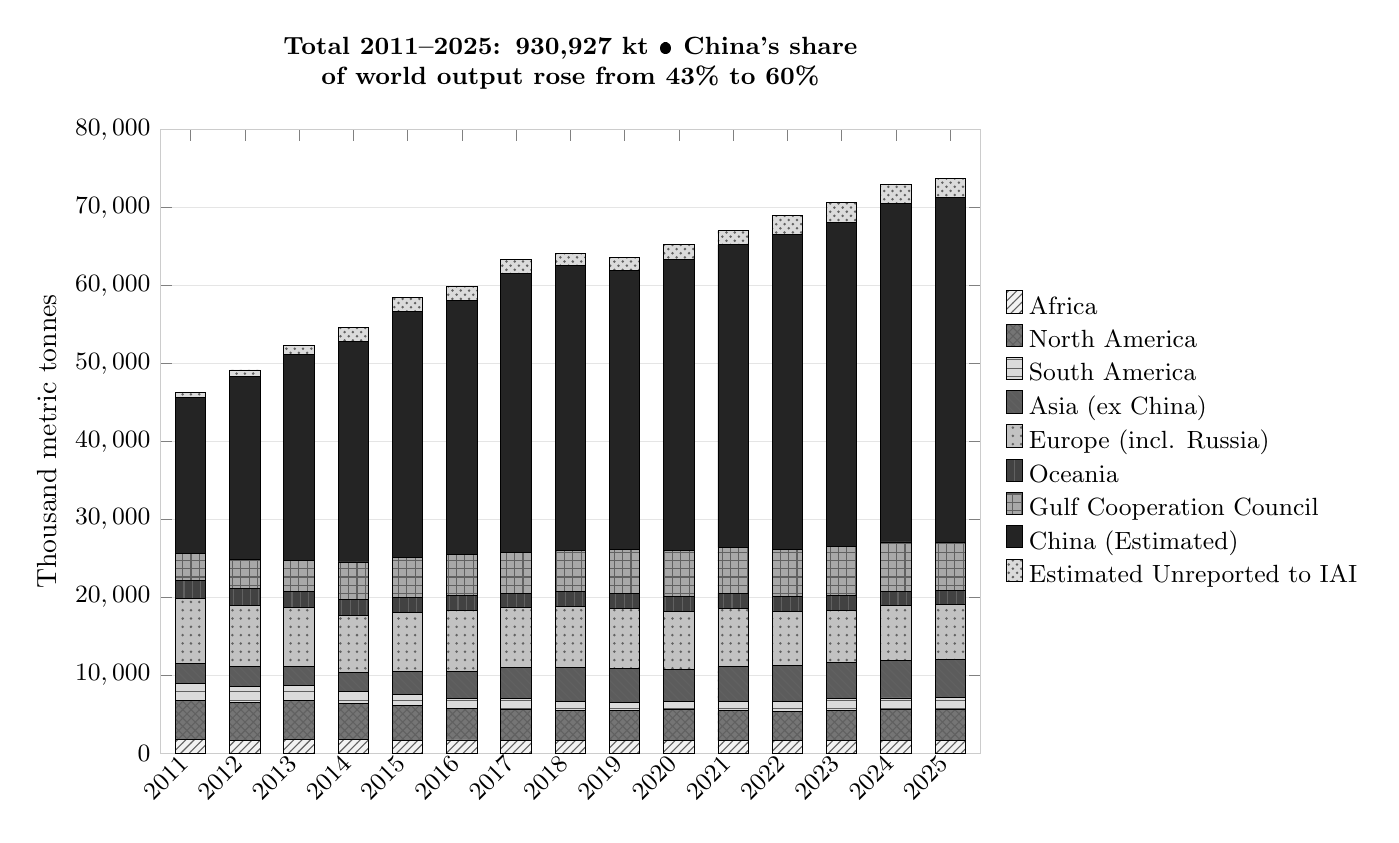
\begin{tikzpicture}
    \begin{axis}[
        ybar stacked,
        width=12cm,
        height=9.5cm,
        bar width=11pt,
        title={\textbf{Total 2011--2025: 930{,}927 kt \textbullet\ China's share of world output rose from 43\% to 60\%}},
        title style={yshift=5pt, font=\small\bfseries, align=center, text width=11cm},
        ylabel={Thousand metric tonnes},
        ymin=0, ymax=80000,
        ytick={0,10000,20000,30000,40000,50000,60000,70000,80000},
        scaled y ticks=false,
        yticklabel style={/pgf/number format/fixed, /pgf/number format/1000 sep={,}, font=\small},
        xtick={2011,2012,2013,2014,2015,2016,2017,2018,2019,2020,2021,2022,2023,2024,2025},
        x tick label style={/pgf/number format/1000 sep={}, rotate=45, anchor=east, font=\small},
        enlarge x limits=0.04,
        ymajorgrids=true,
        major grid style={gray!20},
        axis line style={gray!40},
        legend style={at={(1.02,0.5)}, anchor=west, legend columns=1, draw=none, font=\small},
        legend cell align={left},
    ]
    \addplot[fill=g1, draw=black, line width=0.35pt, postaction={pattern=north east lines, pattern color=black!62}] coordinates {(2011,1805) (2012,1639) (2013,1812) (2014,1746) (2015,1687) (2016,1691) (2017,1679) (2018,1668) (2019,1643) (2020,1605) (2021,1590) (2022,1620) (2023,1594) (2024,1576) (2025,1615)};
    \addlegendentry{Africa}

    \addplot[fill=g6, draw=black, line width=0.35pt, postaction={pattern=crosshatch, pattern color=black!62}] coordinates {(2011,4969) (2012,4851) (2013,4918) (2014,4585) (2015,4469) (2016,4027) (2017,3950) (2018,3774) (2019,3809) (2020,3976) (2021,3880) (2022,3743) (2023,3897) (2024,3983) (2025,3938)};
    \addlegendentry{North America}

    \addplot[fill=g2, draw=black, line width=0.35pt, postaction={pattern=horizontal lines, pattern color=black!62}] coordinates {(2011,2185) (2012,2052) (2013,1906) (2014,1543) (2015,1325) (2016,1361) (2017,1378) (2018,1164) (2019,1079) (2020,1006) (2021,1163) (2022,1288) (2023,1466) (2024,1521) (2025,1551)};
    \addlegendentry{South America}

    \addplot[fill=g7, draw=black, line width=0.35pt, postaction={pattern=north west lines, pattern color=black!62}] coordinates {(2011,2533) (2012,2535) (2013,2439) (2014,2429) (2015,3001) (2016,3442) (2017,3951) (2018,4415) (2019,4395) (2020,4140) (2021,4499) (2022,4591) (2023,4673) (2024,4812) (2025,4859)};
    \addlegendentry{Asia (ex China)}

    \addplot[fill=g3, draw=black, line width=0.35pt, postaction={pattern=dots, pattern color=black!62}] coordinates {(2011,8346) (2012,7928) (2013,7611) (2014,7360) (2015,7574) (2016,7760) (2017,7775) (2018,7782) (2019,7606) (2020,7487) (2021,7468) (2022,6994) (2023,6729) (2024,6996) (2025,7059)};
    \addlegendentry{Europe (incl. Russia)}

    \addplot[fill=g8, draw=black, line width=0.35pt, postaction={pattern=vertical lines, pattern color=black!62}] coordinates {(2011,2306) (2012,2186) (2013,2104) (2014,2035) (2015,1978) (2016,1971) (2017,1817) (2018,1917) (2019,1916) (2020,1912) (2021,1888) (2022,1843) (2023,1884) (2024,1863) (2025,1878)};
    \addlegendentry{Oceania}

    \addplot[fill=g4, draw=black, line width=0.35pt, postaction={pattern=grid, pattern color=black!62}] coordinates {(2011,3483) (2012,3662) (2013,3887) (2014,4832) (2015,5104) (2016,5197) (2017,5149) (2018,5331) (2019,5654) (2020,5833) (2021,5889) (2022,6074) (2023,6217) (2024,6346) (2025,6159)};
    \addlegendentry{Gulf Cooperation Council}

    \addplot[fill=g9, draw=black, line width=0.35pt] coordinates {(2011,20072) (2012,23534) (2013,26534) (2014,28317) (2015,31518) (2016,32641) (2017,35905) (2018,36485) (2019,35795) (2020,37337) (2021,38837) (2022,40430) (2023,41666) (2024,43396) (2025,44219)};
    \addlegendentry{China (Estimated)}

    \addplot[fill=g2, draw=black, line width=0.35pt, postaction={pattern=crosshatch dots, pattern color=black!62}] coordinates {(2011,576) (2012,780) (2013,1080) (2014,1800) (2015,1800) (2016,1800) (2017,1800) (2018,1630) (2019,1760) (2020,2029) (2021,1878) (2022,2455) (2023,2590) (2024,2516) (2025,2516)};
    \addlegendentry{Estimated Unreported to IAI}

    \end{axis}
    \end{tikzpicture}%
    }

    \vspace{0.2cm}
    \raggedright
    \small Source: International Aluminium Institute (IAI); annual totals of monthly reported primary aluminium production. Data for Jan--May 2026 are available but omitted for year-on-year comparability. From 2020 onward the IAI reports European output on a combined ``Europe (incl.\ Russia)'' basis; earlier ``Western \& Central'' and ``Russia \& Eastern'' figures are aggregated here for a consistent series.
\end{figure}

Within India, the influx of primary aluminium is highly concentrated among a few key trading partners. An analysis of the top exporting countries of primary aluminum to India reveals that nations such as Malaysia, the United Arab Emirates, Qatar, and Bahrain thoroughly dominate the import volume (see Figure \ref{fig:top_exporters})\footnote{Source: ITC Trade Map.}. This concentration clearly underscores the impact of Preferential Trade Agreements (PTAs) in the region and necessitates a critical review of the current tariff structures to protect domestic downstream manufacturers.

\begin{figure}[H]
    \centering
    \captionsetup{font={color=black, normalsize}, justification=centering}
    \caption{Top Exporting Countries of Primary Aluminum to India in 2021 (Tons)}
    \label{fig:top_exporters}
    \vspace{0.5cm}

    \resizebox{\textwidth}{!}{%
    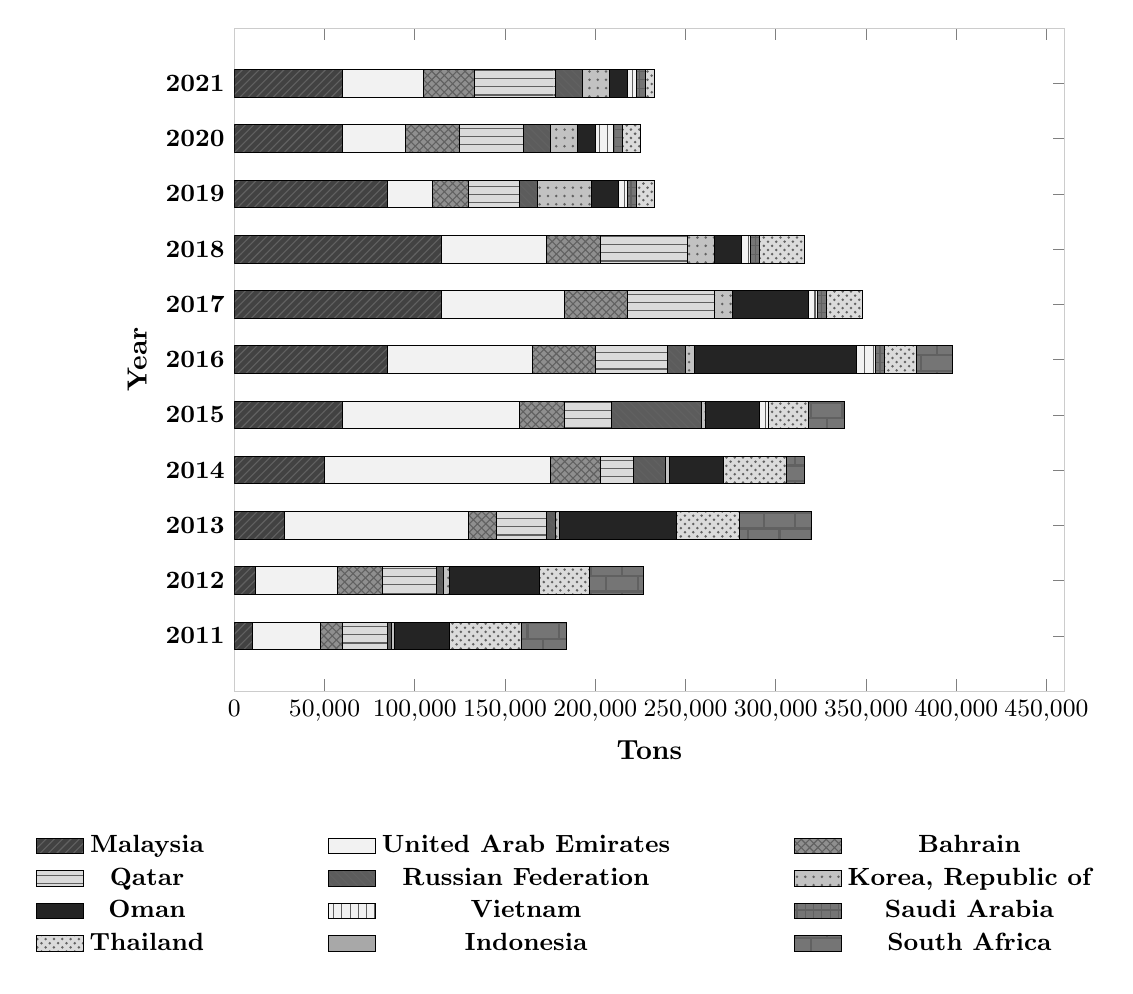
\begin{tikzpicture}
        \begin{axis}[
            xbar stacked,
            width=\textwidth,
            height=10cm,
            bar width=10pt,
            xmin=0,
            xmax=460000,
            xtick={0, 50000, 100000, 150000, 200000, 250000, 300000, 350000, 400000, 450000},
            scaled x ticks=false,
            xticklabel style={/pgf/number format/fixed, font=\small\bfseries},
            xlabel={\textbf{Tons}},
            ylabel={\textbf{Year}},
            yticklabel style={font=\small\bfseries},
            symbolic y coords={2011,2012,2013,2014,2015,2016,2017,2018,2019,2020,2021},
            ytick=data,
            axis line style={gray!40},
            legend style={
                at={(0.4,-0.2)},
                anchor=north,
                legend columns=3,
                draw=none,
                font=\small\bfseries,
                /tikz/every even column/.append style={column sep=1.5cm}
            },
            area legend
        ]

        \addplot[fill=g8, draw=black, line width=0.35pt, postaction={pattern=north east lines, pattern color=black!62}] coordinates {(10000,2011) (12000,2012) (28000,2013) (50000,2014) (60000,2015) (85000,2016) (115000,2017) (115000,2018) (85000,2019) (60000,2020) (60000,2021)};
        \addlegendentry{Malaysia}

        \addplot[fill=g1, draw=black, line width=0.35pt] coordinates {(38000,2011) (45000,2012) (102000,2013) (125000,2014) (98000,2015) (80000,2016) (68000,2017) (58000,2018) (25000,2019) (35000,2020) (45000,2021)};
        \addlegendentry{United Arab Emirates}

        \addplot[fill=g5, draw=black, line width=0.35pt, postaction={pattern=crosshatch, pattern color=black!62}] coordinates {(12000,2011) (25000,2012) (15000,2013) (28000,2014) (25000,2015) (35000,2016) (35000,2017) (30000,2018) (20000,2019) (30000,2020) (28000,2021)};
        \addlegendentry{Bahrain}

        \addplot[fill=g2, draw=black, line width=0.35pt, postaction={pattern=horizontal lines, pattern color=black!62}] coordinates {(25000,2011) (30000,2012) (28000,2013) (18000,2014) (26000,2015) (40000,2016) (48000,2017) (48000,2018) (28000,2019) (35000,2020) (45000,2021)};
        \addlegendentry{Qatar}

        \addplot[fill=g7, draw=black, line width=0.35pt, postaction={pattern=north west lines, pattern color=black!62}] coordinates {(2000,2011) (4000,2012) (5000,2013) (18000,2014) (50000,2015) (10000,2016) (0,2017) (0,2018) (10000,2019) (15000,2020) (15000,2021)};
        \addlegendentry{Russian Federation}

        \addplot[fill=g3, draw=black, line width=0.35pt, postaction={pattern=dots, pattern color=black!62}] coordinates {(2000,2011) (3000,2012) (2000,2013) (2000,2014) (2000,2015) (5000,2016) (10000,2017) (15000,2018) (30000,2019) (15000,2020) (15000,2021)};
        \addlegendentry{Korea, Republic of}

        \addplot[fill=g9, draw=black, line width=0.35pt] coordinates {(30000,2011) (50000,2012) (65000,2013) (30000,2014) (30000,2015) (90000,2016) (42000,2017) (15000,2018) (15000,2019) (10000,2020) (10000,2021)};
        \addlegendentry{Oman}

        \addplot[fill=g1, draw=black, line width=0.35pt, postaction={pattern=vertical lines, pattern color=black!62}] coordinates {(0,2011) (0,2012) (0,2013) (0,2014) (5000,2015) (10000,2016) (5000,2017) (5000,2018) (5000,2019) (10000,2020) (5000,2021)};
        \addlegendentry{Vietnam}

        \addplot[fill=g6, draw=black, line width=0.35pt, postaction={pattern=grid, pattern color=black!62}] coordinates {(0,2011) (0,2012) (0,2013) (0,2014) (0,2015) (5000,2016) (5000,2017) (5000,2018) (5000,2019) (5000,2020) (5000,2021)};
        \addlegendentry{Saudi Arabia}

        \addplot[fill=g2, draw=black, line width=0.35pt, postaction={pattern=crosshatch dots, pattern color=black!62}] coordinates {(40000,2011) (28000,2012) (35000,2013) (35000,2014) (22000,2015) (18000,2016) (20000,2017) (25000,2018) (10000,2019) (10000,2020) (5000,2021)};
        \addlegendentry{Thailand}

        \addplot[fill=g4, draw=black, line width=0.35pt] coordinates {(0,2011) (0,2012) (0,2013) (0,2014) (0,2015) (0,2016) (0,2017) (0,2018) (0,2019) (0,2020) (0,2021)};
        \addlegendentry{Indonesia}

        \addplot[fill=g6, draw=black, line width=0.35pt, postaction={pattern=bricks, pattern color=black!62}] coordinates {(25000,2011) (30000,2012) (40000,2013) (10000,2014) (20000,2015) (20000,2016) (0,2017) (0,2018) (0,2019) (0,2020) (0,2021)};
        \addlegendentry{South Africa}

        \end{axis}
    \end{tikzpicture}%
    }

    \vspace{1.5cm}
    \raggedright
    Source: ITC Trade Map
\end{figure}

\subsection{Supply-Chain Fragility: Geopolitical Chokepoints, War-Risk Insurance, and Energy Costs}
The heavy import concentration shown above is not just a matter of tariff arithmetic. It is a strategic vulnerability. Because the Inverted Duty Structure pushes domestic fabricators toward imported primary metal and scrap, it simultaneously exposes them to a chain of hidden, non-tariff costs that spike precisely when supply is most stressed. Roughly 60\% of the Gulf Cooperation Council's 5.2 million tonnes of annual primary output is exported globally, and the primary maritime exit route is the Persian Gulf via the Strait of Hormuz—a chokepoint through which around 20\% of the world's oil and LNG also transits\footnote{``The Hidden Tax on Gulf Metal: How Marine War Premiums Are Rewriting the Economics of GCC Aluminium.'' \textit{Discovery Alert} (2026). See also the synthesised trade-cost analysis in Ref.~\cite{costreg2026}.}. Given that Gulf producers—alongside Malaysia—dominate India's import basket, any disruption in this corridor transmits directly into the cost base of Indian downstream MSMEs.

Marine war-risk insurance is the sharpest of these hidden costs. Unlike standard hull or cargo cover, war-risk insurance in designated high-risk zones is priced dynamically by the Lloyd's Joint War Committee: underwriters reassess risk within 24-to-48-hour windows and issue rolling seven-day policies\footnote{\textit{Discovery Alert} (2026); see also \textit{Comprehensive Economic Analysis of the Global Downstream Aluminium Industry} (2026), Ref.~\cite{costreg2026}.}. During periods of escalation the premium has climbed from a nominal fraction of hull value to as much as ten times its baseline, and these weekly surcharges pass immediately from shipowners to charterers and ultimately to aluminium buyers. Crucially, this dynamic decouples physical delivery costs from the London Metal Exchange (LME) headline: during recent Middle-East escalation, LME cash prices actually softened (retreating from roughly USD 3,680 to USD 3,480 per tonne as Chinese exports flooded warehouses) even as the Main Japanese Ports physical premium was projected to surge 27--30\% to USD 450--460 per tonne\footnote{\textit{Comprehensive Economic Analysis of the Global Downstream Aluminium Industry} (2026), Ref.~\cite{costreg2026}. The divergence illustrates that hedging LME exposure alone leaves the downstream buyer fully exposed to physical-premium volatility that cannot be hedged on the exchange.}. For a price-taking Indian MSME, the practical consequence is that the landed cost of imported metal can climb sharply even while the ``headline'' aluminium price is falling.

Pandemic-style logistics shocks and direct energy exposure only compound this fragility. The COVID-19 disruption demonstrated how container shortages, port congestion, and freight-rate spikes can strand raw-material shipments and inflate regional premiums for months at a time—a systemic risk borne disproportionately by small fabricators without the balance sheet to hold buffer inventory or to self-insure. On the energy side, downstream remelting, casting, rolling, and extrusion are thermally intensive and typically fired by natural gas and LPG; fabricators therefore carry structural energy surcharges pegged to volatile gas indices, alongside diesel-linked fuel surcharges on the heavy, oversized freight that finished profiles and coils require\footnote{\textit{Comprehensive Economic Analysis of the Global Downstream Aluminium Industry} (2026), Ref.~\cite{costreg2026}. Fuel surcharges are quoted dynamically (e.g., per hundredweight against national diesel indices) and can swing materially month-to-month, while energy surcharges tier upward automatically once gas indices breach programmatic thresholds.}. In aggregate, these logistics and energy liabilities mean the true cost of relying on imported primary aluminium is both higher and far more volatile than the nominal tariff suggests—strengthening, not weakening, the case for a domestic value chain insulated from these shocks.

\begin{table}[H]
    \centering
    \caption{Indian Downstream Sector: Primary vs. Secondary Aluminium Input Proportions}
    \label{tab:aluminium_shares}
    \begin{tabular}{lcc}
        \toprule
        \textbf{Fiscal Year} & \textbf{Primary (Unwrought) Share} & \textbf{Secondary (Scrap) Share} \\
        \midrule
        FY15 & 69\% & 31\% \\
        FY16 & 73\% & 27\% \\
        FY17 & 72\% & 28\% \\
        FY18 & 69\% & 31\% \\
        FY19 & 66\% & 34\% \\
        FY20 & 64\% & 36\% \\
        FY21 & 60\% & 40\% \\
        FY22 & 57\% & 43\% \\
        FY23 & 61\% & 39\% \\
        FY24 & 62\% & 38\% \\
        \bottomrule
    \end{tabular}
    \vspace{0.5cm}

    \raggedright
    \small \textbf{Note:} Over the past ten fiscal years, the Indian downstream sector has demonstrated a clear pivot toward higher utilization of secondary aluminium. This data is corroborated by reports from CRISIL and the Ministry of Mines, based on a comprehensive review of domestic consumption data. The rising secondary share underscores the sector's growing reliance on imported scrap (HS 7602)—cargo equally exposed to the marine war-risk and freight surcharges described above.
\end{table}

\section{Effective Rate of Protection and the role of Inverted Duty Structure}

\subsection{The Current Tariff Regime, Import Volumes, and the Role of FTAs}
The Indian downstream aluminium sector suffers from a severe Inverted Duty Structure (IDS), which is actively exacerbated by Free Trade Agreements (FTAs) and Preferential Trade Agreements (PTAs). India imported \$1.03 billion worth of unwrought primary aluminium (HS 7601) in 2024, totaling approximately 392,000 tons. Concurrently, India faces a massive influx of downstream imports, with China alone accounting for roughly 70\% of downstream products (such as foils and plates) entering the country \cite{mom_vision2025}\footnote{Ministry of Mines, Government of India. (2025). \textit{Vision Document on Aluminium Metal for India}.}.

The core of the IDS lies in the stark tariff differentials embedded within trade agreements. Primary aluminium (HS 7601) attracts a basic customs duty of 7.5\% (effectively 8.25\% with surcharges). However, finished goods from partners under the ASEAN-India Trade in Goods Agreement (AITIGA) and Comprehensive Economic Partnership Agreements (CEPA) with South Korea and the UAE often enter at 0\% duty.

Crucially, these agreements are heavily skewed against Indian MSMEs. While India placed most downstream items in the "Normal Track" allowing duty-free access, partner nations have shielded their own markets. For instance, Malaysia imposes excessively high Most Favoured Nation (MFN) duties (25\% to 30\%) on tariff lines between 7604 and 7608, and Indonesia places downstream products under "Sensitive Tracks" \cite{mom_vision2025}\footnote{Ministry of Mines, \textit{Vision Document on Aluminium Metal for India} (2025).}. This creates a one-way street where foreign nations can import raw aluminium from India, add value, and dump finished goods back into the Indian market duty-free, completely crippling the competitiveness of domestic manufacturers.

Two domestic factors make the distortion worse still, by inflating the price of the raw input itself. First, because the primary smelting sector is highly consolidated—with a Herfindahl-Hirschman Index exceeding 3,100—upstream producers exploit the 8.25\% tariff wall to practice \textit{import-parity pricing} (IPP), benchmarking domestic prices to the LME plus the import duty and logistics premiums and thereby sustaining a persistent spread of roughly Rs 30,000 to Rs 60,000 per tonne over international prices\footnote{\textit{Comprehensive Economic Analysis of the Global Downstream Aluminium Industry} (2026), Ref.~\cite{costreg2026}. The tariff, originally intended to protect domestic smelters, thus functions as an artificial pricing anchor that the downstream sector is forced to pay.}. Second, statutory levies on energy and minerals—most notably the GST Compensation Cess on coal (escalated over the past decade to INR 400 per tonne) and, following the Supreme Court's August 2024 ruling, retrospective state-level mineral cesses such as Odisha's ORISED and Jharkhand's MADA frameworks—inflate upstream production costs that are then passed down the chain via IPP\footnote{\textit{Comprehensive Economic Analysis of the Global Downstream Aluminium Industry} (2026), Ref.~\cite{costreg2026}. Analysts estimate the mineral-cess ruling alone could raise landed raw-material costs by around 11\% and compress downstream fabricator margins by 80--250 basis points, against a sector that already averages only \textasciitilde5\% margins.}. The combined effect is stark: Indian downstream capacity utilization has fallen to approximately 65\% while consolidated upstream smelters run at close to 98\%.

There is a further channel of cost volatility that tends to go unnoticed, and it sits inside the import-parity formula itself. Because domestic primary prices are constructed as the London Metal Exchange quotation plus a physical premium and a notional customs duty, and then converted into rupees at the prevailing US-dollar exchange rate, any depreciation of the rupee is mechanically passed through into the price paid by the downstream fabricator---even though the metal is produced entirely within India and the primary producer's own costs, incurred in rupees, are unchanged. The inverted duty structure thus acquires a currency dimension: the import-parity model effectively transfers exchange-rate risk on \emph{domestically produced} metal onto the downstream sector, so that a weaker rupee or a firmer LME raises input costs immediately, whereas a transparent, cost-based domestic benchmark would leave them unaffected. For thin-margin MSMEs, which earn in rupees and hold no natural dollar revenues against which to hedge, this currency-linked escalation compounds the margin compression already imposed by the duty inversion and the statutory cesses described above.

\subsection{The Case for Countervailing and Anti-Dumping Measures against Subsidised Imports}
The IDS does not operate in a vacuum; it is weaponised by trading partners—above all China—whose downstream exporters enjoy state support that Indian MSMEs cannot match. A 2019 study by the Organisation for Economic Co-operation and Development (OECD), reviewed in the European Commission's Joint Research Centre assessment of the aluminium sector, found that government support pervades the entire aluminium value chain: each of the 17 largest global producers examined received financial or non-financial support, with five Chinese firms alone capturing over 85\% of documented subsidies estimated at USD 20--70 billion across 2013--2017, largely in the form of energy subsidies and concessional finance\footnote{Georgitzikis, K., Nita, V., Ciupagea, C., \& Garbossa, E. (2021). \textit{The aftermath of US tariffs on aluminium imports: An assessment of tariff impacts and a review of the EU aluminium industry.} EUR 30730 EN, Joint Research Centre, European Commission, Luxembourg. \cite{jrc2021}; drawing on OECD (2019), \textit{Measuring distortions in international markets: the aluminium value chain}. \cite{oecd2019}.}.

What matters most for the Indian case is that China's distortion is deliberately built to favour its \textit{downstream} sector at the direct expense of foreign fabricators. Beijing maintains an export tax of roughly 15\% on primary aluminium and scrap while simultaneously granting a VAT rebate of 13--15\% on exports of semi-finished and fabricated products (rolled products and extrusions)\footnote{Georgitzikis et al.~(2021), EU JRC, and OECD (2019). The export tax discourages the outflow of primary metal, making it artificially cheap to Chinese semis producers, while the VAT rebate subsidises the export of the value-added product—a textbook mechanism for capturing downstream value from competitors.}. The intent was demonstrated in May 2015, when China selectively eliminated its 15\% export tax on certain semi-processed bars, rods, and strip while retaining the 30\% export duty on most primary products; global producer share prices fell almost immediately, while the share price of China's largest state-owned producer rose by around 10\%\footnote{DeFrancesco, R.~E., \& Teslik, A.~M. (2015). \textit{China's Selective Elimination of Aluminum Export Duties Threatens Global Manufacturers.} Wiley Rein LLP Alert. \cite{wiley2015}.}. This subsidy architecture, combined with structural overcapacity (Chinese primary output rose from 11\% of world supply in 2000 to 56\% in 2019, with idle smelting capacity exceeding 13 Mt), is precisely what floods the Indian market with below-cost foils and plates.

The right response to subsidised and dumped imports is not tariff rationalisation alone. It is the active use of the trade-remedy instruments the WTO framework already permits—anti-dumping duties on demonstrably below-cost imports and countervailing duties calibrated to neutralise the quantified foreign subsidy. India's downstream sector, unlike its trading partners, has been slow to seek such protection; a proactive regime of countervailing measures targeting subsidised Chinese and ASEAN semi-finished goods would restore competitive symmetry and complement the tariff reforms recommended in Section~5.

\subsection{Empirical Evidence: The Erosion of Effective Protection, 2015--16 to 2024--25}
The Effective Rate of Protection (ERP) provides the most appropriate empirical tool for analysing an Inverted Duty Structure. Whereas a nominal tariff records only the duty on the finished good, the ERP measures the protection afforded to the \emph{value added} in a productive process, netting out the tariffs paid on that process's own intermediate inputs. Where input duties exceed output duties, the measure turns negative: the tariff regime taxes domestic transformation rather than protecting it, a paradox documented for Indian manufacturing more broadly by Pathania and Bhattacharjea \cite{pathania2020}\footnote{Pathania, K., \& Bhattacharjea, A. (2020). \textit{Inverted Duty Structures and the Paradox of Negative Effective Protection in India, 2000-2014.} Foreign Trade Review, 55(2), 139--167.}.

\subsubsection*{Data and method}
We estimate ERP for thirteen downstream product lines (HS 7604--7616) against six trading partners, at three points in time: 2015--16, 2019--20 and 2024--25. Estimates apply the modified Corden formulation set out in Appendix~A, using Ministry of Statistics and Programme Implementation (MOSPI) Supply Use Tables for the input--output coefficients, and partner-specific applied (preferential where an agreement is in force, MFN otherwise) tariff schedules for output and import-weighted input duties. Looking at three widely spaced years rather than a single baseline lets us watch successive trade agreements take effect as they phase in.

\begin{table}[H]
    \centering
    \caption{Effective Rate of Protection by downstream product line, 2024--25 (per cent)}
    \label{tab:erp_2024}
    \resizebox{\textwidth}{!}{
    \begin{tabular}{llrrrrrr}
        \toprule
        \textbf{Output Product} & \textbf{HS Code} & \textbf{Malaysia} & \textbf{S.~Korea} & \textbf{Japan} & \textbf{Thailand} & \textbf{UAE} & \textbf{UK} \\
        \midrule
        Bars, Rods \& Profiles & 7604 & $-2.0$ & $-2.0$ & $-2.0$ & $-2.0$ & $+6.0$ & $+38.0$ \\
        Wires \& Cables & 7605 & $-1.0$ & $-1.0$ & $-1.0$ & $-1.0$ & $+7.0$ & $+38.0$ \\
        Flat Rolled Products & 7606 & $-2.0$ & $-2.0$ & $-2.0$ & $-2.0$ & $+6.0$ & $+37.0$ \\
        Aluminium Foils & 7607 & $-5.0$ & $-5.0$ & $-5.0$ & $-5.0$ & $+3.0$ & $+34.0$ \\
        Tubes and Pipes & 7608 & $-1.0$ & $-1.0$ & $-1.0$ & $-1.0$ & $+9.0$ & $+51.0$ \\
        Tube/Pipe Fittings & 7609 & $-3.0$ & $-3.0$ & $-3.0$ & $-3.0$ & $+8.0$ & $+50.0$ \\
        Aluminium Structures & 7610 & $-2.0$ & $-2.0$ & $-2.0$ & $-2.0$ & $+9.0$ & $+51.0$ \\
        Reservoirs, Tanks, Vats & 7611 & $-1.0$ & $-1.0$ & $-1.0$ & $-1.0$ & $+9.0$ & $+51.0$ \\
        Casks, Drums \& Cans & 7612 & $-3.0$ & $-3.0$ & $-3.0$ & $-3.0$ & $+8.0$ & $+50.0$ \\
        Containers for Gas & 7613 & $-4.0$ & $-4.0$ & $-4.0$ & $-4.0$ & $+6.0$ & $+48.0$ \\
        Stranded Wire, Cables & 7614 & $-1.0$ & $-0.5$ & $-0.5$ & $-0.5$ & $+10.0$ & $+52.0$ \\
        Utensils & 7615 & $-6.0$ & $-6.0$ & $-6.0$ & $-6.0$ & $+15.0$ & $+99.0$ \\
        Castings & 7616 & $-6.0$ & $-6.0$ & $-6.0$ & $-6.0$ & $+4.0$ & $+46.0$ \\
        \midrule
        \textbf{Simple average} & & $\mathbf{-2.9}$ & $\mathbf{-2.8}$ & $\mathbf{-2.8}$ & $\mathbf{-2.8}$ & $\mathbf{+7.7}$ & $\mathbf{+49.6}$ \\
        \bottomrule
    \end{tabular}
    }

    \vspace{0.2cm}
    \raggedright
    \small \textbf{Note:} Our estimates. A negative value denotes \emph{disprotection}: the tariff structure leaves domestic value added lower than it would be under free trade. The UK column reflects MFN treatment during the estimation year and is reported as a non-preferential benchmark; the exceptionally high figure for utensils (HS 7615) reflects that line's unusually low input-to-output value ratio and should be read with caution.
\end{table}

The result in Table~\ref{tab:erp_2024} is strikingly uniform. In 2024--25, every single one of the fifty-two product--partner combinations involving Malaysia, South Korea, Japan and Thailand shows a negative ERP. This is not a quirk of one product line or one partner: it runs across the whole downstream range, from simple extrusions right through to finished utensils and castings.

\subsubsection*{The trend: protection erodes as agreements phase in}
What the three estimation years reveal when set side by side is more telling still. Table~\ref{tab:erp_trend} and Figure~\ref{fig:erp_trend} summarise the comparison.

\begin{table}[H]
    \centering
    \caption{Average ERP across thirteen downstream product lines, by partner and period (per cent)}
    \label{tab:erp_trend}
    \begin{tabular}{lrrr}
        \toprule
        \textbf{Partner} & \textbf{2015--16} & \textbf{2019--20} & \textbf{2024--25} \\
        \midrule
        Malaysia & $-4.1$ & $-2.9$ & $-2.9$ \\
        South Korea & $+10.2$ & $-2.9$ & $-2.8$ \\
        Japan & $+23.0$ & $+5.1$ & $-2.8$ \\
        Thailand & $-5.0$ & $-2.9$ & $-2.8$ \\
        UAE & $+42.3$ & $+54.4$ & $+7.7$ \\
        UK (non-preferential benchmark) & $+42.4$ & $+54.4$ & $+49.6$ \\
        \midrule
        \multicolumn{4}{l}{\textit{Product--partner cells with negative ERP, preferential partners only:}} \\
        Malaysia, S.~Korea, Japan, Thailand & 26 of 52 & 34 of 52 & \textbf{52 of 52} \\
        \bottomrule
    \end{tabular}

    \vspace{0.2cm}
    \raggedright
    \small \textbf{Note:} Simple (unweighted) averages of the thirteen product-line estimates. Our calculations.
\end{table}

Three things stand out here, and they matter more than any single-year snapshot could show.

\begin{enumerate}
    \item \textbf{Preferential partners have moved from positive to negative protection.} South Korea's average ERP fell from $+10.2$\% in 2015--16 to $-2.9$\% by 2019--20; Japan's fell from $+23.0$\% to $+5.1$\% and then to $-2.8$\%. Malaysia and Thailand were already negative in 2015--16 and have remained so. The count of negative product--partner cells rose from 26 of 52, to 34 of 52, to all 52.
    \item \textbf{The UAE illustrates the mechanism directly.} Effective protection against UAE-origin goods stood at $+42.3$\% in 2015--16 and $+54.4$\% in 2019--20. Following the India--UAE Comprehensive Economic Partnership Agreement, it collapsed to $+7.7$\% in 2024--25---a fall of roughly forty-seven percentage points, with no corresponding reduction in the duty payable on the sector's primary input.
    \item \textbf{The contrast with a non-preferential benchmark is the control.} The United Kingdom, trading on MFN terms across these years, retained an average ERP of $+49.6$\% in 2024--25. The divergence between this benchmark and the preferential columns isolates the effect of the agreements themselves rather than of any general change in India's tariff schedule.
\end{enumerate}

\begin{figure}[H]
    \centering
    \captionsetup{font={color=black, normalsize}, justification=centering}
    \caption{Average Effective Rate of Protection by partner and period}
    \label{fig:erp_trend}
    \vspace{0.3cm}

    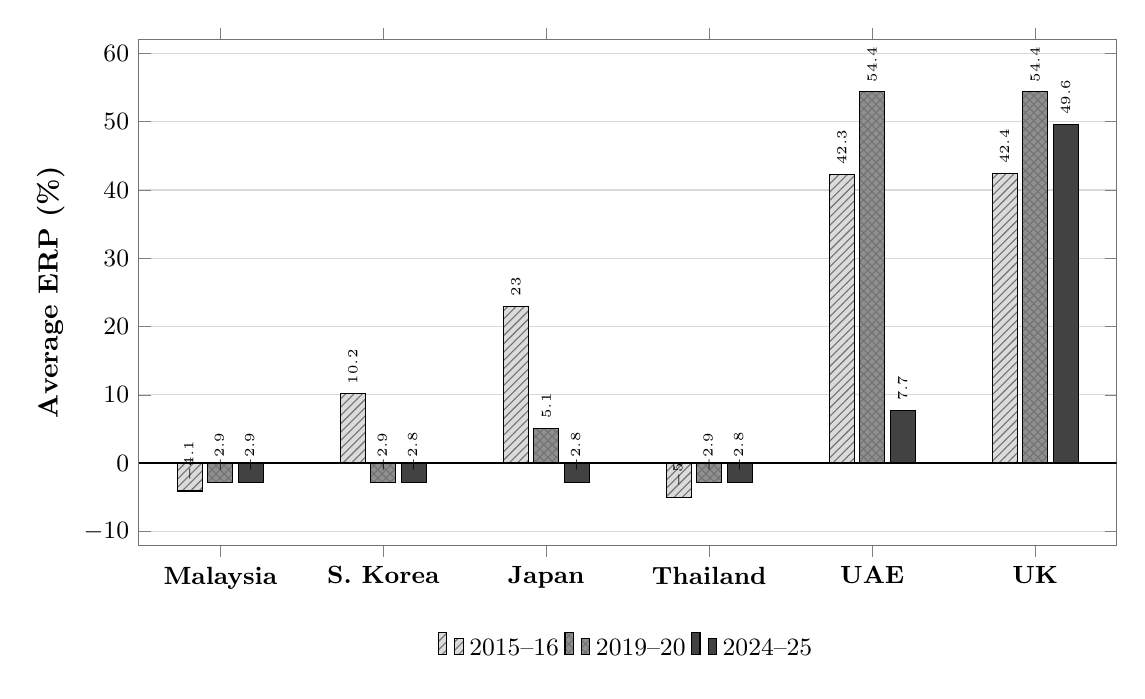
\begin{tikzpicture}
    \begin{axis}[
        ybar,
        width=14cm, height=8cm,
        bar width=9pt,
        ymin=-12, ymax=62,
        ytick={-10,0,10,20,30,40,50,60},
        ylabel={\textbf{Average ERP (\%)}},
        symbolic x coords={Malaysia,{S. Korea},Japan,Thailand,UAE,UK},
        xtick=data,
        x tick label style={font=\small\bfseries},
        tick label style={font=\small},
        ymajorgrids=true, major grid style={black!15},
        axis line style={black!55},
        legend style={at={(0.5,-0.16)}, anchor=north, legend columns=3, draw=none, font=\small},
        legend cell align={left},
        nodes near coords={\pgfmathprintnumber[fixed, precision=1]\pgfplotspointmeta},
        every node near coord/.append style={font=\tiny, rotate=90, anchor=west},
    ]
    \addplot[fill=g2, draw=black, line width=0.4pt, postaction={pattern=north east lines, pattern color=black!55}]
      coordinates {(Malaysia,-4.08) ({S. Korea},10.15) (Japan,23.00) (Thailand,-5.00) (UAE,42.31) (UK,42.38)};
    \addlegendentry{2015--16}
    \addplot[fill=g5, draw=black, line width=0.4pt, postaction={pattern=crosshatch, pattern color=black!55}]
      coordinates {(Malaysia,-2.85) ({S. Korea},-2.85) (Japan,5.08) (Thailand,-2.85) (UAE,54.38) (UK,54.38)};
    \addlegendentry{2019--20}
    \addplot[fill=g8, draw=black, line width=0.4pt]
      coordinates {(Malaysia,-2.85) ({S. Korea},-2.81) (Japan,-2.81) (Thailand,-2.81) (UAE,7.69) (UK,49.62)};
    \addlegendentry{2024--25}
    \draw[black, thick] ({rel axis cs:0,0}|-{axis cs:Malaysia,0}) -- ({rel axis cs:1,0}|-{axis cs:Malaysia,0});
    \end{axis}
    \end{tikzpicture}

    \vspace{0.2cm}
    \raggedright
    \small Source: Our estimates from MOSPI Supply Use Tables and partner tariff schedules. Bars below the zero line denote negative effective protection. The UK series is a non-preferential (MFN) benchmark.
\end{figure}

Read together, these estimates point to something more troubling than a one-off distortion. The disprotection facing India's downstream aluminium sector is not standing still---it is widening, and it widens in step with the order in which India's trade agreements have come into force.

\subsection{The "Lose-Lose" Scenario for the Indian Consumer}
As established in trade literature, increased access to imported intermediate varieties is a primary driver of domestic product scope expansion and innovation \cite{goldberg2010}\footnote{Goldberg, P. K., Khandelwal, A. K., Pavcnik, N., \& Topalova, P. (2010). \textit{Imported Intermediate Inputs and Domestic Product Growth: Evidence from India.} The Quarterly Journal of Economics, 125(4), 1727--1767.}. By maintaining high input tariffs, the current policy stifles domestic product diversification. This creates a "lose-lose" scenario for the Indian consumer:
\begin{enumerate}
    \item \textbf{Vulnerable Supply Chains:} Consumers become overly reliant on imported finished goods from PTA nations and China, reducing domestic supply chain resilience.
    \item \textbf{Stifled Innovation:} High costs for intermediate inputs deprive consumers of new, customized domestic product varieties.
    \item \textbf{Eroded Purchasing Power:} The destruction of the labour-intensive MSME downstream sector results in widespread job losses, directly impacting the economic well-being of the Indian working class.
\end{enumerate}

\section{Policy Plight of MSMEs in the Aluminium Industry}

\subsection{Measuring the Sector: NIC Concordance and ASI Definitions}
\label{sec:asi_method}
The claims made so far deserve to be tested against official statistics rather than industry assertion. To do that, we turn to aggregates from the \textbf{Annual Survey of Industries (ASI)}, the principal source of industrial statistics for India's registered factory sector, compiled by the National Statistical Office \cite{asi2024}\footnote{National Statistical Office, Ministry of Statistics and Programme Implementation, Government of India. \textit{Annual Survey of Industries}, All-India summary results, 2011--12 to 2023--24.}. Activities are mapped to the National Industrial Classification (NIC) 2008 at the four-digit level, following the concordance in Table~\ref{tab:nic_concordance} \cite{nic2008}\footnote{Central Statistical Organisation, \textit{National Industrial Classification (NIC) 2008}, Government of India.}.

\begin{table}[H]
    \centering
    \caption{NIC 2008 concordance for the aluminium value chain}
    \label{tab:nic_concordance}
    \begin{tabular}{llp{7.6cm}l}
        \toprule
        \textbf{Phase} & \textbf{NIC} & \textbf{Description of industrial activity} & \textbf{Metal} \\
        \midrule
        Upstream & 0729 & Mining of aluminium ore (bauxite) & Aluminium \\
        Upstream & 2420 & Manufacture of aluminium from alumina and products & Aluminium \\
        \midrule
        Downstream & 2432 & Casting of non-ferrous metals & Aluminium/Both \\
        Downstream & 2511 & Manufacture of structural metal products (frameworks, doors) & Aluminium \\
        Downstream & 2599 & Manufacture of metal household articles and utensils & Aluminium/Both \\
        Downstream & 2710 & Manufacture of electric motors, generators, transformers & Aluminium/Both \\
        Downstream & 2732 & Manufacture of electronic and electric wires and cables & Aluminium/Both \\
        Downstream & 3030 & Manufacture of air and spacecraft & Aluminium \\
        \bottomrule
    \end{tabular}

    \vspace{0.2cm}
    \raggedright
    \small \textbf{Scope note.} NIC~0729 (bauxite mining) lies outside the ASI frame, which covers registered manufacturing only; the upstream aggregate below therefore comprises NIC~2420. Classes marked ``Aluminium/Both'' are not exclusive to aluminium---they are the classes in which aluminium fabrication is concentrated but which also contain other non-ferrous and ferrous activity. The downstream aggregate should accordingly be read as \emph{the registered manufacturing space within which downstream aluminium activity sits}, not as a pure aluminium account. This is a deliberate and conservative choice: no attempt is made to apportion these classes by metal, which would require assumptions the published data cannot support.
\end{table}

The ASI variables used carry their standard published definitions. \textit{Gross Value Added} is total output less total input; it is reported here at current prices, with \textbf{no deflator applied}, so the growth rates below are nominal and overstate real expansion. \textit{Total Persons Engaged} comprises all workers, employees other than workers, and unpaid family members or proprietors. \textit{Total Workers} decomposes into those \textit{directly employed} and those \textit{employed through contractors}. \textit{Employees other than workers} splits into supervisory/managerial and other employees. Corporate tax is not published directly and is estimated as net profit multiplied by the effective corporate tax rate prevailing in each year; because a negative net profit yields a meaningless negative tax, \textbf{loss-making observations are excluded} from the tax series rather than netted off.\footnote{Three observations are affected: NIC~2733 and 3030 in 2011--12 and NIC~2432 in 2013--14. Excluding rather than netting them avoids reporting a negative tax contribution that has no behavioural interpretation.}

\subsection{Gross Value Added: Comparable Growth, Divergent Employment}
Over the thirteen years to 2023--24 the two segments generated almost identical nominal GVA growth. Upstream GVA rose 178.3 per cent and downstream GVA 178.2 per cent---a compound annual rate of 8.9 per cent in both cases (Figure~\ref{fig:asi_index}). In level terms the downstream aggregate remains substantially the larger of the two, at INR 1,16,966 crore against INR 49,801 crore upstream in 2023--24.

\begin{figure}[H]
    \centering
    \captionsetup{font={color=black, normalsize}, justification=centering}
    \caption{Gross Value Added and Persons Engaged, index 2011--12 $=$ 100}
    \label{fig:asi_index}
    \vspace{0.3cm}

    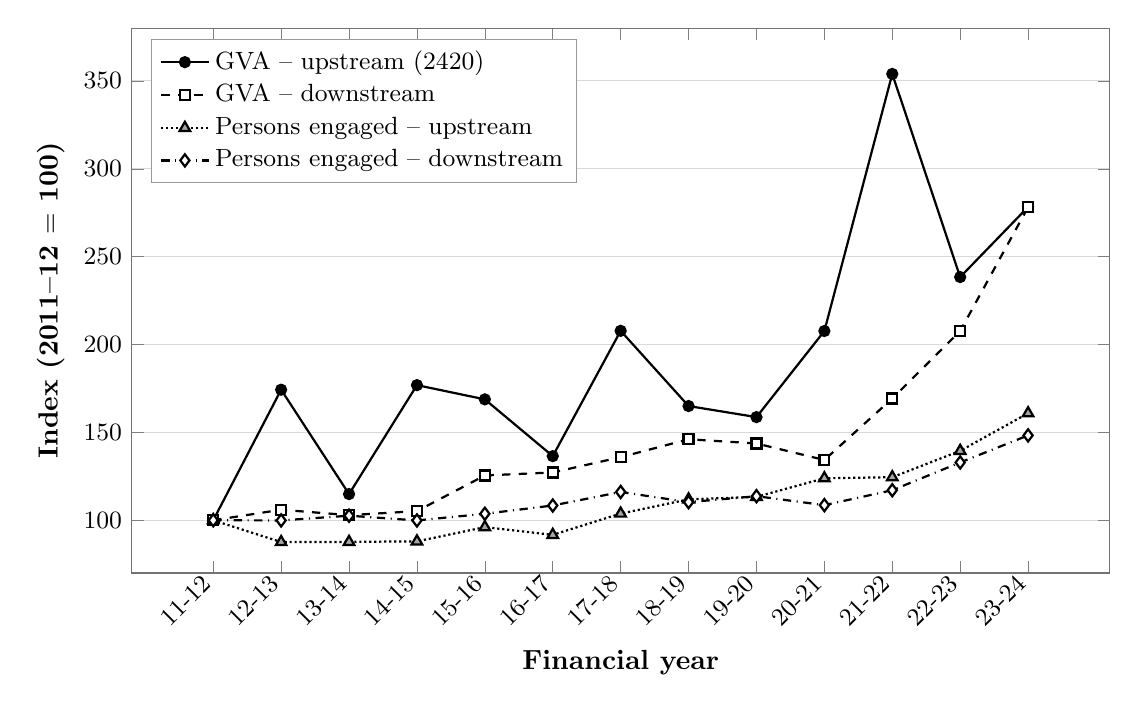
\begin{tikzpicture}
    \begin{axis}[
        width=14cm, height=8.5cm,
        ymin=70, ymax=380,
        ylabel={\textbf{Index (2011--12 $=$ 100)}},
        xlabel={\textbf{Financial year}},
        symbolic x coords={11-12,12-13,13-14,14-15,15-16,16-17,17-18,18-19,19-20,20-21,21-22,22-23,23-24},
        xtick=data,
        x tick label style={rotate=45, anchor=east, font=\small},
        tick label style={font=\small},
        ymajorgrids=true, major grid style={black!15},
        axis line style={black!55},
        legend style={at={(0.02,0.98)}, anchor=north west, draw=black!40, fill=white, font=\small},
        legend cell align={left},
        cycle list name=black white,
    ]
    \addplot[black, thick, mark=*, mark size=1.8pt] coordinates {(11-12,100.0)(12-13,174.3)(13-14,114.9)(14-15,176.9)(15-16,168.8)(16-17,136.5)(17-18,207.8)(18-19,165.0)(19-20,158.7)(20-21,207.7)(21-22,354.0)(22-23,238.4)(23-24,278.3)};
    \addlegendentry{GVA -- upstream (2420)}
    \addplot[black, thick, dashed, mark=square*, mark size=1.8pt, mark options={solid, fill=white}] coordinates {(11-12,100.0)(12-13,106.0)(13-14,102.9)(14-15,105.2)(15-16,125.5)(16-17,127.2)(17-18,135.9)(18-19,146.1)(19-20,143.7)(20-21,134.3)(21-22,169.3)(22-23,207.7)(23-24,278.2)};
    \addlegendentry{GVA -- downstream}
    \addplot[black, densely dotted, thick, mark=triangle*, mark size=2.2pt, mark options={solid, fill=black!35}] coordinates {(11-12,100.0)(12-13,87.6)(13-14,87.7)(14-15,88.0)(15-16,96.1)(16-17,91.7)(17-18,103.8)(18-19,111.9)(19-20,113.3)(20-21,123.9)(21-22,124.5)(22-23,139.5)(23-24,160.9)};
    \addlegendentry{Persons engaged -- upstream}
    \addplot[black, dashdotted, thick, mark=diamond*, mark size=2.2pt, mark options={solid, fill=white}] coordinates {(11-12,100.0)(12-13,99.9)(13-14,102.6)(14-15,99.9)(15-16,103.7)(16-17,108.4)(17-18,116.1)(18-19,110.3)(19-20,113.7)(20-21,108.6)(21-22,117.1)(22-23,132.9)(23-24,148.3)};
    \addlegendentry{Persons engaged -- downstream}
    \end{axis}
    \end{tikzpicture}

    \vspace{0.2cm}
    \raggedright
    \small Source: Our calculations from ASI All-India summary results. GVA at current prices (nominal; no deflator applied). Upstream $=$ NIC~2420; downstream $=$ NIC~2432, 2511, 2599, 2710, 2732, 3030.
\end{figure}

What makes this equivalence interesting is what it costs in employment terms. Upstream GVA is generated by a workforce of 197,170 persons; the downstream aggregate engages 1,006,275---some \textbf{5.1 times} as many people for value added that is, in growth terms, expanding at the same rate. Expressed per head, upstream value added stood at INR 25.3 lakh per person engaged in 2023--24 against INR 11.6 lakh downstream (Figure~\ref{fig:asi_gpp}). Each rupee of downstream value added therefore sustains roughly \textbf{2.2 times} more employment than the same rupee generated upstream.

\begin{figure}[H]
    \centering
    \captionsetup{font={color=black, normalsize}, justification=centering}
    \caption{Gross Value Added per person engaged (INR lakh, current prices)}
    \label{fig:asi_gpp}
    \vspace{0.3cm}

    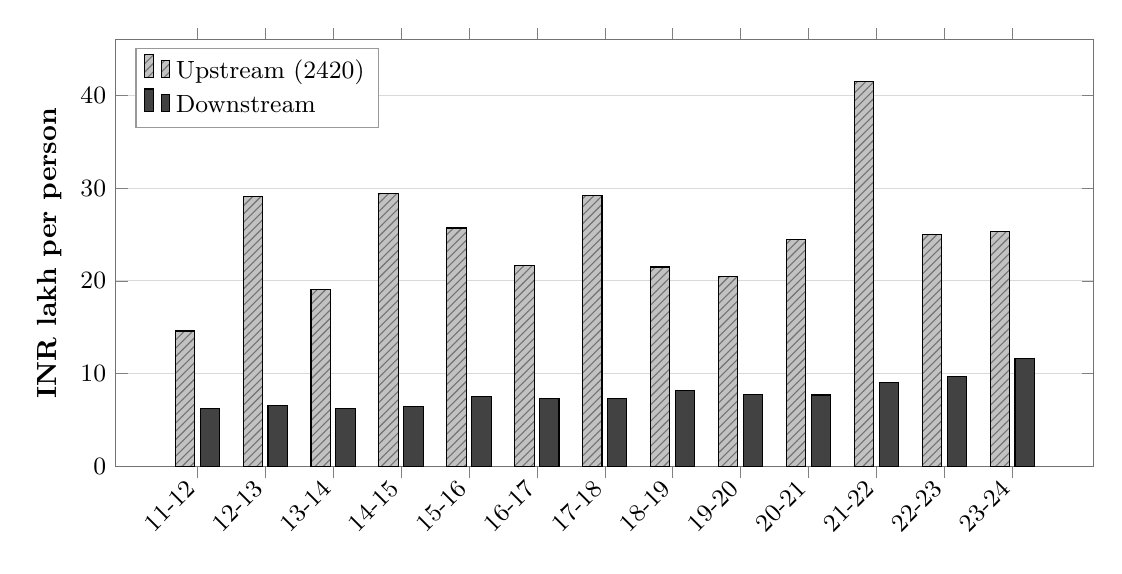
\begin{tikzpicture}
    \begin{axis}[
        ybar,
        width=14cm, height=7cm,
        bar width=7pt,
        ymin=0, ymax=46,
        ylabel={\textbf{INR lakh per person}},
        symbolic x coords={11-12,12-13,13-14,14-15,15-16,16-17,17-18,18-19,19-20,20-21,21-22,22-23,23-24},
        xtick=data,
        x tick label style={rotate=45, anchor=east, font=\small},
        tick label style={font=\small},
        ymajorgrids=true, major grid style={black!15},
        axis line style={black!55},
        legend style={at={(0.02,0.98)}, anchor=north west, draw=black!40, fill=white, font=\small},
        legend cell align={left},
    ]
    \addplot[fill=g3, draw=black, line width=0.4pt, postaction={pattern=north east lines, pattern color=black!55}]
      coordinates {(11-12,14.6)(12-13,29.1)(13-14,19.1)(14-15,29.4)(15-16,25.7)(16-17,21.7)(17-18,29.2)(18-19,21.5)(19-20,20.5)(20-21,24.5)(21-22,41.5)(22-23,25.0)(23-24,25.3)};
    \addlegendentry{Upstream (2420)}
    \addplot[fill=g8, draw=black, line width=0.4pt]
      coordinates {(11-12,6.2)(12-13,6.6)(13-14,6.2)(14-15,6.5)(15-16,7.5)(16-17,7.3)(17-18,7.3)(18-19,8.2)(19-20,7.8)(20-21,7.7)(21-22,9.0)(22-23,9.7)(23-24,11.6)};
    \addlegendentry{Downstream}
    \end{axis}
    \end{tikzpicture}

    \vspace{0.2cm}
    \raggedright
    \small Source: Our calculations from ASI All-India summary results. A \emph{lower} bar denotes greater labour intensity---more persons engaged per unit of value added.
\end{figure}

This is what people mean, in concrete terms, when they call the downstream segment the employment-intensive node of the value chain. It also corroborates, from an entirely independent source, the Ministry of Mines' assessment that downstream activity can generate two-and-a-half to three times the employment of primary production \cite{mom_vision2025}\footnote{Ministry of Mines, \textit{Vision Document on Aluminium Metal for India} (2025).}; our own ASI-based estimate of 2.2 times per unit of value added lands in the same territory. We report the lower figure rather than the higher one, simply because it is what the official data will bear.

\subsection{Employment Dynamics: Pro-Employer Labour Intensity}
The downstream manufacturing of end-consumer products---utensils, architectural fittings, auto components---is inherently labour-intensive. Unlike the highly capital-intensive and mechanised upstream smelting process, the downstream segment is the crucial node for large-scale job creation in India, a proposition Figure~\ref{fig:asi_gpp} quantifies.

Breaking the record down by NIC class, as Table~\ref{tab:asi_growth} does, reveals a picture that is uneven in ways that matter a great deal for policy. Two downstream classes closely associated with construction and consumer goods have performed poorly: structural metal products (NIC~2511) grew GVA by only 28.5 per cent over thirteen nominal years---far below inflation, implying a substantial real contraction---while its contract workforce fell 47.2 per cent and its estimated tax contribution declined 12.6 per cent. That is the profile of a segment under sustained competitive pressure---and it happens to be exactly the segment most exposed to duty-free finished imports.

\begin{table}[H]
    \centering
    \caption{Percentage change by NIC class, 2011--12 to 2023--24}
    \label{tab:asi_growth}
    \resizebox{\textwidth}{!}{
    \begin{tabular}{lrrrrr}
        \toprule
        \textbf{NIC class} & \textbf{GVA} & \textbf{Persons engaged} & \textbf{Total workers} & \textbf{Contract workers} & \textbf{Corporate tax} \\
        \midrule
        \multicolumn{6}{l}{\textit{Upstream}} \\
        2420 Primary aluminium & $+178.3$ & $+60.9$ & $+70.1$ & $+5.5$ & $+223.0$ \\
        \midrule
        \multicolumn{6}{l}{\textit{Downstream}} \\
        2432 Casting of non-ferrous metals & $+228.4$ & $+65.6$ & $+68.2$ & $+0.3$ & $+303.9$ \\
        2511 Structural metal products & $+28.5$ & $+1.7$ & $+0.6$ & $-47.2$ & $-12.6$ \\
        2599 Other fabricated metal products & $+284.3$ & $+59.0$ & $+59.0$ & $-8.1$ & $+406.6$ \\
        2710 Motors, generators, transformers & $+166.4$ & $+37.0$ & $+50.2$ & $+38.9$ & $+262.3$ \\
        2732 Other wires and cables & $+385.3$ & $+161.2$ & $+188.3$ & $+72.6$ & $+736.5$ \\
        3030 Air and spacecraft & $+1{,}923.8$ & $+500.1$ & $+443.5$ & $+892.6$ & n.a. \\
        \midrule
        \textbf{Upstream total} & $\mathbf{+178.3}$ & $\mathbf{+60.9}$ & $\mathbf{+70.1}$ & $\mathbf{+5.5}$ & $\mathbf{+223.0}$ \\
        \textbf{Downstream total} & $\mathbf{+178.2}$ & $\mathbf{+48.3}$ & $\mathbf{+52.9}$ & $\mathbf{+1.0}$ & $\mathbf{+223.9}$ \\
        \bottomrule
    \end{tabular}
    }

    \vspace{0.2cm}
    \raggedright
    \small Source: Our calculations from ASI All-India summary results. All values nominal (current prices). ``n.a.'' for NIC~3030 corporate tax: the 2011--12 base observation was loss-making and is excluded, leaving no valid base for a percentage change. NIC~3030 is a small class expanding from a very low base, and its percentages should be read accordingly.
\end{table}

The composition of the workforce reinforces the argument advanced by Chaurey \cite{chaurey2015}\footnote{Chaurey, R. (2015). \textit{Labor regulations and contract labor use: Evidence from Indian firms.} Journal of Development Economics, 114, 224--232.} that Indian manufacturers rely on contract labour to navigate the rigidities of employment protection legislation such as the Industrial Disputes Act, 1947. Because permanent workers are difficult to adjust during market fluctuations, firms use contract workers as the margin of flexibility. Figure~\ref{fig:asi_contract} shows that in both segments contract workers constitute roughly two-fifths to one-half of the total workforce throughout the period---in downstream aluminium fabrication, a stable 39.3 to 44.1 per cent.

\begin{figure}[H]
    \centering
    \captionsetup{font={color=black, normalsize}, justification=centering}
    \caption{Workers employed through contractors as a share of total workers (per cent)}
    \label{fig:asi_contract}
    \vspace{0.3cm}

    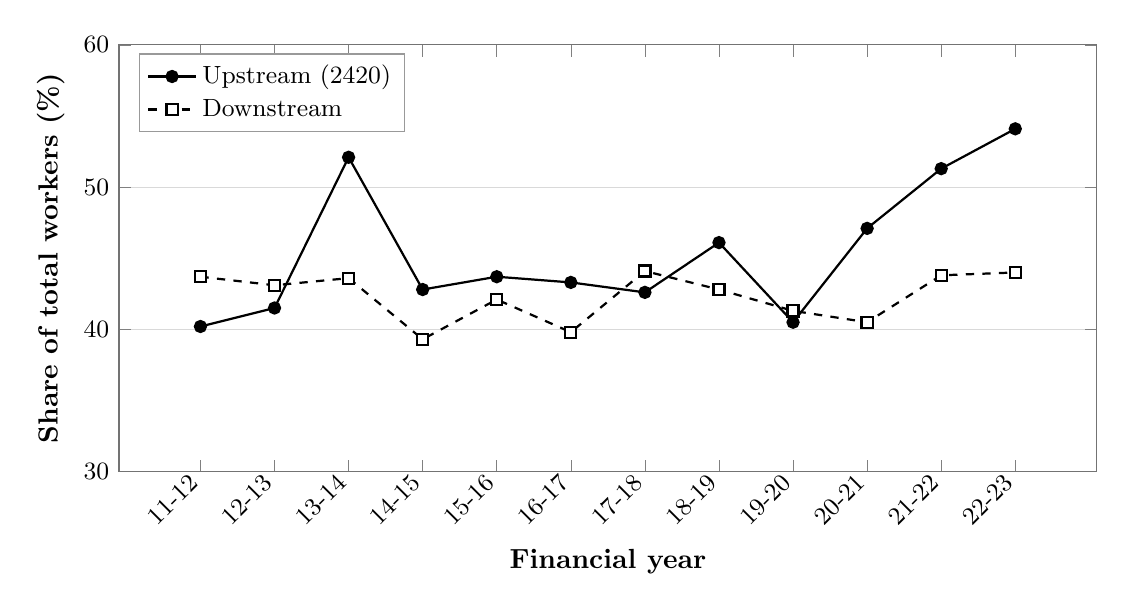
\begin{tikzpicture}
    \begin{axis}[
        width=14cm, height=7cm,
        ymin=30, ymax=60,
        ylabel={\textbf{Share of total workers (\%)}},
        xlabel={\textbf{Financial year}},
        symbolic x coords={11-12,12-13,13-14,14-15,15-16,16-17,17-18,18-19,19-20,20-21,21-22,22-23},
        xtick=data,
        x tick label style={rotate=45, anchor=east, font=\small},
        tick label style={font=\small},
        ymajorgrids=true, major grid style={black!15},
        axis line style={black!55},
        legend style={at={(0.02,0.98)}, anchor=north west, draw=black!40, fill=white, font=\small},
        legend cell align={left},
    ]
    \addplot[black, thick, mark=*, mark size=2pt] coordinates {(11-12,40.2)(12-13,41.5)(13-14,52.1)(14-15,42.8)(15-16,43.7)(16-17,43.3)(17-18,42.6)(18-19,46.1)(19-20,40.5)(20-21,47.1)(21-22,51.3)(22-23,54.1)};
    \addlegendentry{Upstream (2420)}
    \addplot[black, thick, dashed, mark=square*, mark size=2pt, mark options={solid, fill=white}] coordinates {(11-12,43.7)(12-13,43.1)(13-14,43.6)(14-15,39.3)(15-16,42.1)(16-17,39.8)(17-18,44.1)(18-19,42.8)(19-20,41.3)(20-21,40.5)(21-22,43.8)(22-23,44.0)};
    \addlegendentry{Downstream}
    \end{axis}
    \end{tikzpicture}

    \vspace{0.2cm}
    \raggedright
    \small Source: Our calculations from ASI All-India summary results. \textbf{2023--24 is omitted:} in that year the published directly-employed and contract-worker counts do not sum to total workers (an aggregate residual of 193,626 workers across the eight classes examined), whereas the identity holds exactly in every year from 2011--12 to 2022--23. The series is therefore truncated rather than presented on an inconsistent basis.
\end{figure}

The policy implication here is hard to miss. Roughly two out of every five downstream workers hold contract rather than permanent status, and contract labour is by construction the first margin of adjustment. When domestic fabricators face an artificial negative demand shock---being undercut by zero-duty finished imports, or absorbing an input-cost spike they cannot pass on---the adjustment falls immediately on this workforce. Trade anomalies at the tariff line are transmitted, with very little lag, into job losses among the least protected participants in the value chain.

\subsection{Corporate Tax: The Downstream Sector's Fiscal Contribution}
One final piece of evidence speaks to the fiscal side of the argument. Estimated corporate tax paid by the downstream classes has risen from INR 3,688 crore in 2011--12 to INR 11,943 crore in 2023--24, overtaking the upstream contribution, which stood at INR 5,061 crore in the same year (Figure~\ref{fig:asi_tax}). The downstream aggregate has exceeded the upstream contribution in each of the two most recent years, 2022--23 and 2023--24; the relative position fluctuates in earlier years, and in 2021--22 the upstream classes recorded the higher figure.

\begin{figure}[H]
    \centering
    \captionsetup{font={color=black, normalsize}, justification=centering}
    \caption{Estimated corporate tax contribution (INR thousand crore)}
    \label{fig:asi_tax}
    \vspace{0.3cm}

    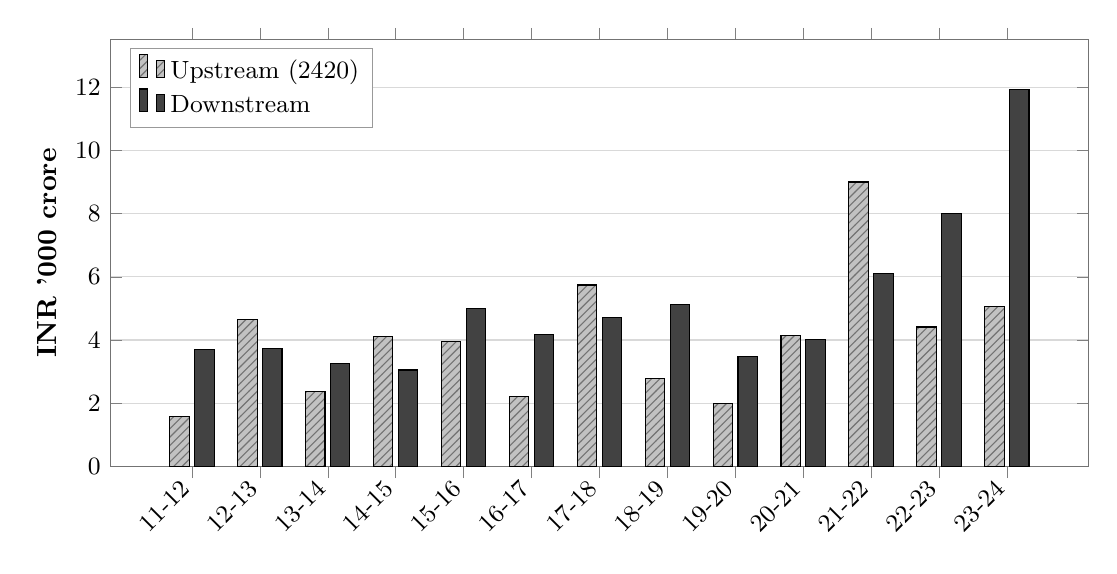
\begin{tikzpicture}
    \begin{axis}[
        ybar,
        width=14cm, height=7cm,
        bar width=7pt,
        ymin=0, ymax=13.5,
        ylabel={\textbf{INR '000 crore}},
        symbolic x coords={11-12,12-13,13-14,14-15,15-16,16-17,17-18,18-19,19-20,20-21,21-22,22-23,23-24},
        xtick=data,
        x tick label style={rotate=45, anchor=east, font=\small},
        tick label style={font=\small},
        ymajorgrids=true, major grid style={black!15},
        axis line style={black!55},
        legend style={at={(0.02,0.98)}, anchor=north west, draw=black!40, fill=white, font=\small},
        legend cell align={left},
    ]
    \addplot[fill=g3, draw=black, line width=0.4pt, postaction={pattern=north east lines, pattern color=black!55}]
      coordinates {(11-12,1.57)(12-13,4.64)(13-14,2.38)(14-15,4.10)(15-16,3.94)(16-17,2.22)(17-18,5.74)(18-19,2.78)(19-20,1.99)(20-21,4.13)(21-22,9.00)(22-23,4.41)(23-24,5.06)};
    \addlegendentry{Upstream (2420)}
    \addplot[fill=g8, draw=black, line width=0.4pt]
      coordinates {(11-12,3.69)(12-13,3.72)(13-14,3.25)(14-15,3.05)(15-16,4.99)(16-17,4.18)(17-18,4.72)(18-19,5.12)(19-20,3.49)(20-21,4.01)(21-22,6.09)(22-23,7.99)(23-24,11.94)};
    \addlegendentry{Downstream}
    \end{axis}
    \end{tikzpicture}

    \vspace{0.2cm}
    \raggedright
    \small Source: Our calculations from ASI All-India summary results. Corporate tax estimated as net profit $\times$ the effective corporate tax rate for each year; loss-making observations excluded rather than netted (see Section~\ref{sec:asi_method}).
\end{figure}

So the fiscal case runs alongside the employment case rather than pulling against it. The segment that generates the larger absolute value added, engages five times the workforce, and now remits the larger corporate tax contribution is the segment that the tariff structure disprotects. Rationalising the duty on primary aluminium would not forgo revenue from a thriving upstream so much as relieve a cost on the larger fiscal and employment base downstream.

\subsection{Compliance Headwinds: CBAM, ESG Norms, and the CAPEX Barrier to Exports}
Even as domestic MSMEs are squeezed at home, their export potential is increasingly constrained by environmental-compliance regimes in destination markets. From January 2026 the European Union's Carbon Border Adjustment Mechanism (CBAM) entered its definitive phase, converting the embedded-carbon content of imported aluminium into a direct financial obligation: importers must surrender certificates equivalent to the EU Emissions Trading System carbon price, and exporters must supply installation-specific, meter-based, third-party-verified emissions data rather than industry averages\footnote{``How to Calculate Embedded Emissions for UK Aluminium Manufacturers.'' \textit{Below280 / Decerna} (2026); European Commission CBAM Regulation (EU) 2023/956. \cite{cbam2026}.}. Where a producer cannot furnish verified data, the customer is assigned punitive region-specific default values calculated from the worst-emitting 10\% of installations—penalising precisely the small Indian fabricators least able to afford sophisticated carbon accounting. A parallel UK CBAM is scheduled from January 2027, and similar ESG-driven disclosure and due-diligence norms are proliferating across OECD markets.

At bottom, this is a capital problem. Because a large share of an aluminium product's embedded carbon is inherited from upstream coal-fired Indian smelting, meaningful decarbonisation requires cost-intensive technology upgrades—greenfield low-emission smelting routes can entail capital expenditure on the order of USD 350 per tonne, more than double conventional processes, and comprehensive sectoral decarbonisation implies multi-billion-dollar investment\footnote{Ministry of Mines / NITI Aayog, \textit{Roadmap for Aluminium Sector Decarbonisation}. \cite{roadmap2025}. The high upfront CAPEX and elevated cost of capital place verified low-carbon compliance out of reach for most MSMEs absent policy support.}. For a fragmented downstream sector already operating on \textasciitilde5\% margins and paying import-parity prices for its metal, the CAPEX required to meet CBAM and ESG thresholds is prohibitive. Unless input costs are rationalised and targeted green-transition finance is extended, these compliance regimes will function as a de facto non-tariff barrier that locks Indian downstream products out of high-value export markets—compounding the domestic damage inflicted by the Inverted Duty Structure.

\section{Conclusion}
To resolve the structural imbalances within India's aluminium ecosystem and safeguard its strategic future, we propose the following targeted policy interventions \cite{mom_vision2025}\footnote{Ministry of Mines, Government of India. (2025). \textit{Vision Document on Aluminium Metal for India}.}:

\begin{itemize}
    \item \textbf{Tariff Rationalization on Primary Inputs:}
    The government must urgently address the Inverted Duty Structure by rationalizing the 7.5\% basic customs duty on unwrought primary aluminium (HS 7601) and associated raw materials. Aligning the duties on these essential inputs with the zero-duty or low-duty finished goods entering under FTAs is necessary to restore a level playing field for domestic secondary manufacturers and MSMEs.

    \item \textbf{Deploy Trade-Remedy Instruments against Subsidised Imports:}
    Beyond tariff realignment, India should proactively invoke WTO-consistent anti-dumping and countervailing duties on demonstrably subsidised and below-cost semi-finished imports—particularly from China, whose 13--15\% VAT rebates and export-tax architecture directly subsidise its downstream exporters. Trade remedies calibrated to the quantified foreign subsidy would neutralise the distortion at source.

    \item \textbf{Renegotiation of Free Trade Agreements (FTAs):}
    Trade agreements with ASEAN nations (specifically Malaysia and Indonesia) must be revisited to address the non-reciprocal tariff barriers. Downstream items currently placed on Sensitive Tracks or subjected to high MFN duties by partner nations must be renegotiated to allow fair market access for Indian MSME exports.

    \item \textbf{Establish a Transparent Domestic Pricing Framework:}
    Currently, primary producers operate on an Import Parity Pricing (IPP) model tied to the London Metal Exchange (LME). This effectively inflates domestic prices despite India's inherent low-cost production advantages. Shifting toward a transparent, cost-based domestic pricing framework will shield downstream MSMEs from global market volatility and severe margin pressures.

    \item \textbf{Enable Green-Transition Finance for CBAM/ESG Compliance:}
    To preserve export access under the EU and UK CBAM and proliferating ESG norms, policymakers should pair input-cost relief with targeted concessional finance and incentives for the high-CAPEX technology upgrades required to produce verified low-carbon aluminium, ensuring MSMEs are not locked out of high-value markets.

    \item \textbf{Streamline Regulatory Burdens and QCOs:}
    Non-tariff barriers, particularly Quality Control Orders (QCOs) on upstream product categories, restrict access to necessary imported raw materials and impose heavy compliance costs on MSMEs. Policymakers must continue to limit QCO burdens on critical intermediate inputs to prevent supply chain disruptions in the downstream sector.
\end{itemize}

Correcting the tariff anomalies and market rigidities facing the downstream aluminium industry is a strategic economic imperative. As India navigates the pressures of global supply chains, geopolitical chokepoints, subsidised foreign competition, rapid urbanization, and the impending EU CBAM, empowering the secondary manufacturing sector is essential. The downstream sector has the capacity to generate nearly triple the employment of the primary sector. By rationalizing input tariffs, deploying trade remedies against subsidised imports, renegotiating unbalanced FTAs, ensuring transparent domestic pricing, enabling green-transition finance, and easing regulatory burdens, policymakers can unlock massive GVA potential. Crucially, these reforms will safeguard the thousands of MSMEs that form the backbone of this industry, thereby protecting and expanding a vital, pro-employer base for India's growing workforce.

\newpage
\begin{thebibliography}{99}

\bibitem{pathania2020}
Pathania, K., \& Bhattacharjea, A. (2020).
\textit{Inverted Duty Structures and the Paradox of Negative Effective Protection in India, 2000-2014.}
Foreign Trade Review, 55(2), 139--167.

\bibitem{goldberg2010}
Goldberg, P. K., Khandelwal, A. K., Pavcnik, N., \& Topalova, P. (2010).
\textit{Imported Intermediate Inputs and Domestic Product Growth: Evidence from India.}
The Quarterly Journal of Economics, 125(4), 1727--1767.

\bibitem{chaurey2015}
Chaurey, R. (2015).
\textit{Labor regulations and contract labor use: Evidence from Indian firms.}
Journal of Development Economics, 114, 224--232.

\bibitem{mom_vision2025}
Ministry of Mines, Government of India. (2025).
\textit{Vision Document on Aluminium Metal for India}.
New Delhi, India.

\bibitem{jrc2021}
Georgitzikis, K., Nita, V., Ciupagea, C., \& Garbossa, E. (2021).
\textit{The aftermath of US tariffs on aluminium imports: An assessment of tariff impacts and a review of the EU aluminium industry.}
EUR 30730 EN, Joint Research Centre, European Commission, Luxembourg. doi:10.2760/46784.

\bibitem{oecd2019}
Organisation for Economic Co-operation and Development. (2019).
\textit{Measuring distortions in international markets: the aluminium value chain.}
OECD Trade Policy Papers, No. 218, OECD Publishing, Paris.

\bibitem{wiley2015}
DeFrancesco, R. E., \& Teslik, A. M. (2015).
\textit{China's Selective Elimination of Aluminum Export Duties Threatens Global Manufacturers.}
Wiley Rein LLP International Trade Alert, May 22, 2015.

\bibitem{cbam2026}
European Commission. (2023).
\textit{Regulation (EU) 2023/956 establishing a Carbon Border Adjustment Mechanism (CBAM).}
Official Journal of the European Union; definitive phase from January 2026.

\bibitem{roadmap2025}
Ministry of Mines / NITI Aayog, Government of India.
\textit{Roadmap for Aluminium Sector Decarbonisation.}
New Delhi, India.

\bibitem{asi2024}
National Statistical Office, Ministry of Statistics and Programme Implementation, Government of India.
\textit{Annual Survey of Industries (ASI)}, All-India summary results, 2011--12 to 2023--24.
New Delhi. Variable definitions per the ASI schedule and published concepts and definitions.

\bibitem{nic2008}
Central Statistical Organisation, Ministry of Statistics and Programme Implementation, Government of India. (2008).
\textit{National Industrial Classification (NIC) 2008.}
New Delhi.

\bibitem{alcircle2026}
AL Circle. (2026).
\textit{Vedanta Aluminium to rally 22\%? Nuvama initiates `Buy' with 29\% EBITDA forecast.}
14 July 2026. https://www.alcircle.com/news/vedanta-aluminium-to-rally-22-nuvama-initiates-buy-with-29-ebitda-forecast-120324

\bibitem{arora2023}
Arora, A. (2023).
\textit{Assessing the Impact of CBAM and Tariffs in the Indian Aluminum Industry.}
IIFT Working Paper Series, WPS No.~EC-23-65, Indian Institute of Foreign Trade, New Delhi.

\bibitem{bensalha2025}
Ben-Salha, O., Zmami, M., Waked, S. S., Najjar, F., \& Alenazi, Y. M. (2025).
\textit{On the time-varying spillover between nonferrous metals prices, geopolitical risks, and global economic policy uncertainty.}
Economic Change and Restructuring, 58(5).

\bibitem{costreg2026}
\textit{Comprehensive Economic Analysis of the Global Downstream Aluminium Industry: Regulatory Frameworks, Cost Modeling, and Supply Chain Mechanics.}
Synthesis of trade data and peer-reviewed literature, 2026.

\end{thebibliography}

\newpage
\appendix
\section{Appendix: Technical Framework of ERP Analysis}
This appendix provides the technical foundation for the Effective Rate of Protection (ERP) calculations presented in Section 3, utilizing the modified approach established by Pathania \& Bhattacharjea (2020) \cite{pathania2020}\footnote{Pathania, K., \& Bhattacharjea, A. (2020). \textit{Inverted Duty Structures and the Paradox of Negative Effective Protection in India, 2000-2014.} Foreign Trade Review, 55(2), 139--167.} to account for domestic price valuations based on Input-Output tables.

\subsection{Modified Corden's Approach}
We utilize a modified formulation of Corden's measure that adapts to the availability of data from the MOSPI Supply Use Tables (SUTs). We define ERP in sector $j$ as:
$$ ERP_j = \frac{VA_{Tj} - VA_{FTj}}{VA_{FTj}} $$
Where $VA_{Tj}$ refers to value added under restricted trade at basic prices, and $VA_{FTj}$ refers to value added under free trade at basic prices.

Using observable SUT data, value added under restricted trade is algebraically represented as:
$$ VA_{Tj} = VO_j - \sum_i IC_{ij} $$
Where:
\begin{itemize}
    \item $VO_j$: Value of the output of sector $j$ at basic prices.
    \item $IC_{ij}$: Intermediate consumption of good $i$ in the production of output $j$ at purchasers' price.
\end{itemize}

To find the counterfactual value added under free trade ($VA_{FTj}$), we deflate the ex-post value of output and intermediate inputs by the rate of tariff charged on each product:
$$ VA_{FTj} = \frac{VO_j}{(1+t_j)} - \sum_i \frac{IC_{ij}}{(1+t_i)} $$
Where:
\begin{itemize}
    \item $t_j$: Nominal ad valorem tariff on the import of final output $j$.
    \item $t_i$: Import-weighted average ad valorem tariff on inputs.
\end{itemize}

Substituting these into the ERP definition yields the operational formula used for our baseline estimations:
$$ ERP_j = \frac{ \left(VO_j - \sum_i IC_{ij}\right) - \left( \frac{VO_j}{1+t_j} - \sum_i \frac{IC_{ij}}{1+t_i} \right) }{ \frac{VO_j}{1+t_j} - \sum_i \frac{IC_{ij}}{1+t_i} } $$

This framework mathematically demonstrates that an Inverted Duty Structure (where $t_i > t_j$, as seen in the Indian downstream aluminium sector under FTAs) directly erodes the domestic value added margin, driving the ERP negative and artificially disprotecting the industry.

\newpage
\section{Appendix: Supplementary Figures}
\label{app:figures}

For consolidated reference, all figures presented in the body of the report are reproduced together below, in the order in which they appear. All charts use a greyscale palette with hatch patterning so that every series remains legible in black-and-white printing or photocopying.

\begin{figure}[H]
    \centering
    \resizebox{\textwidth}{!}{%
    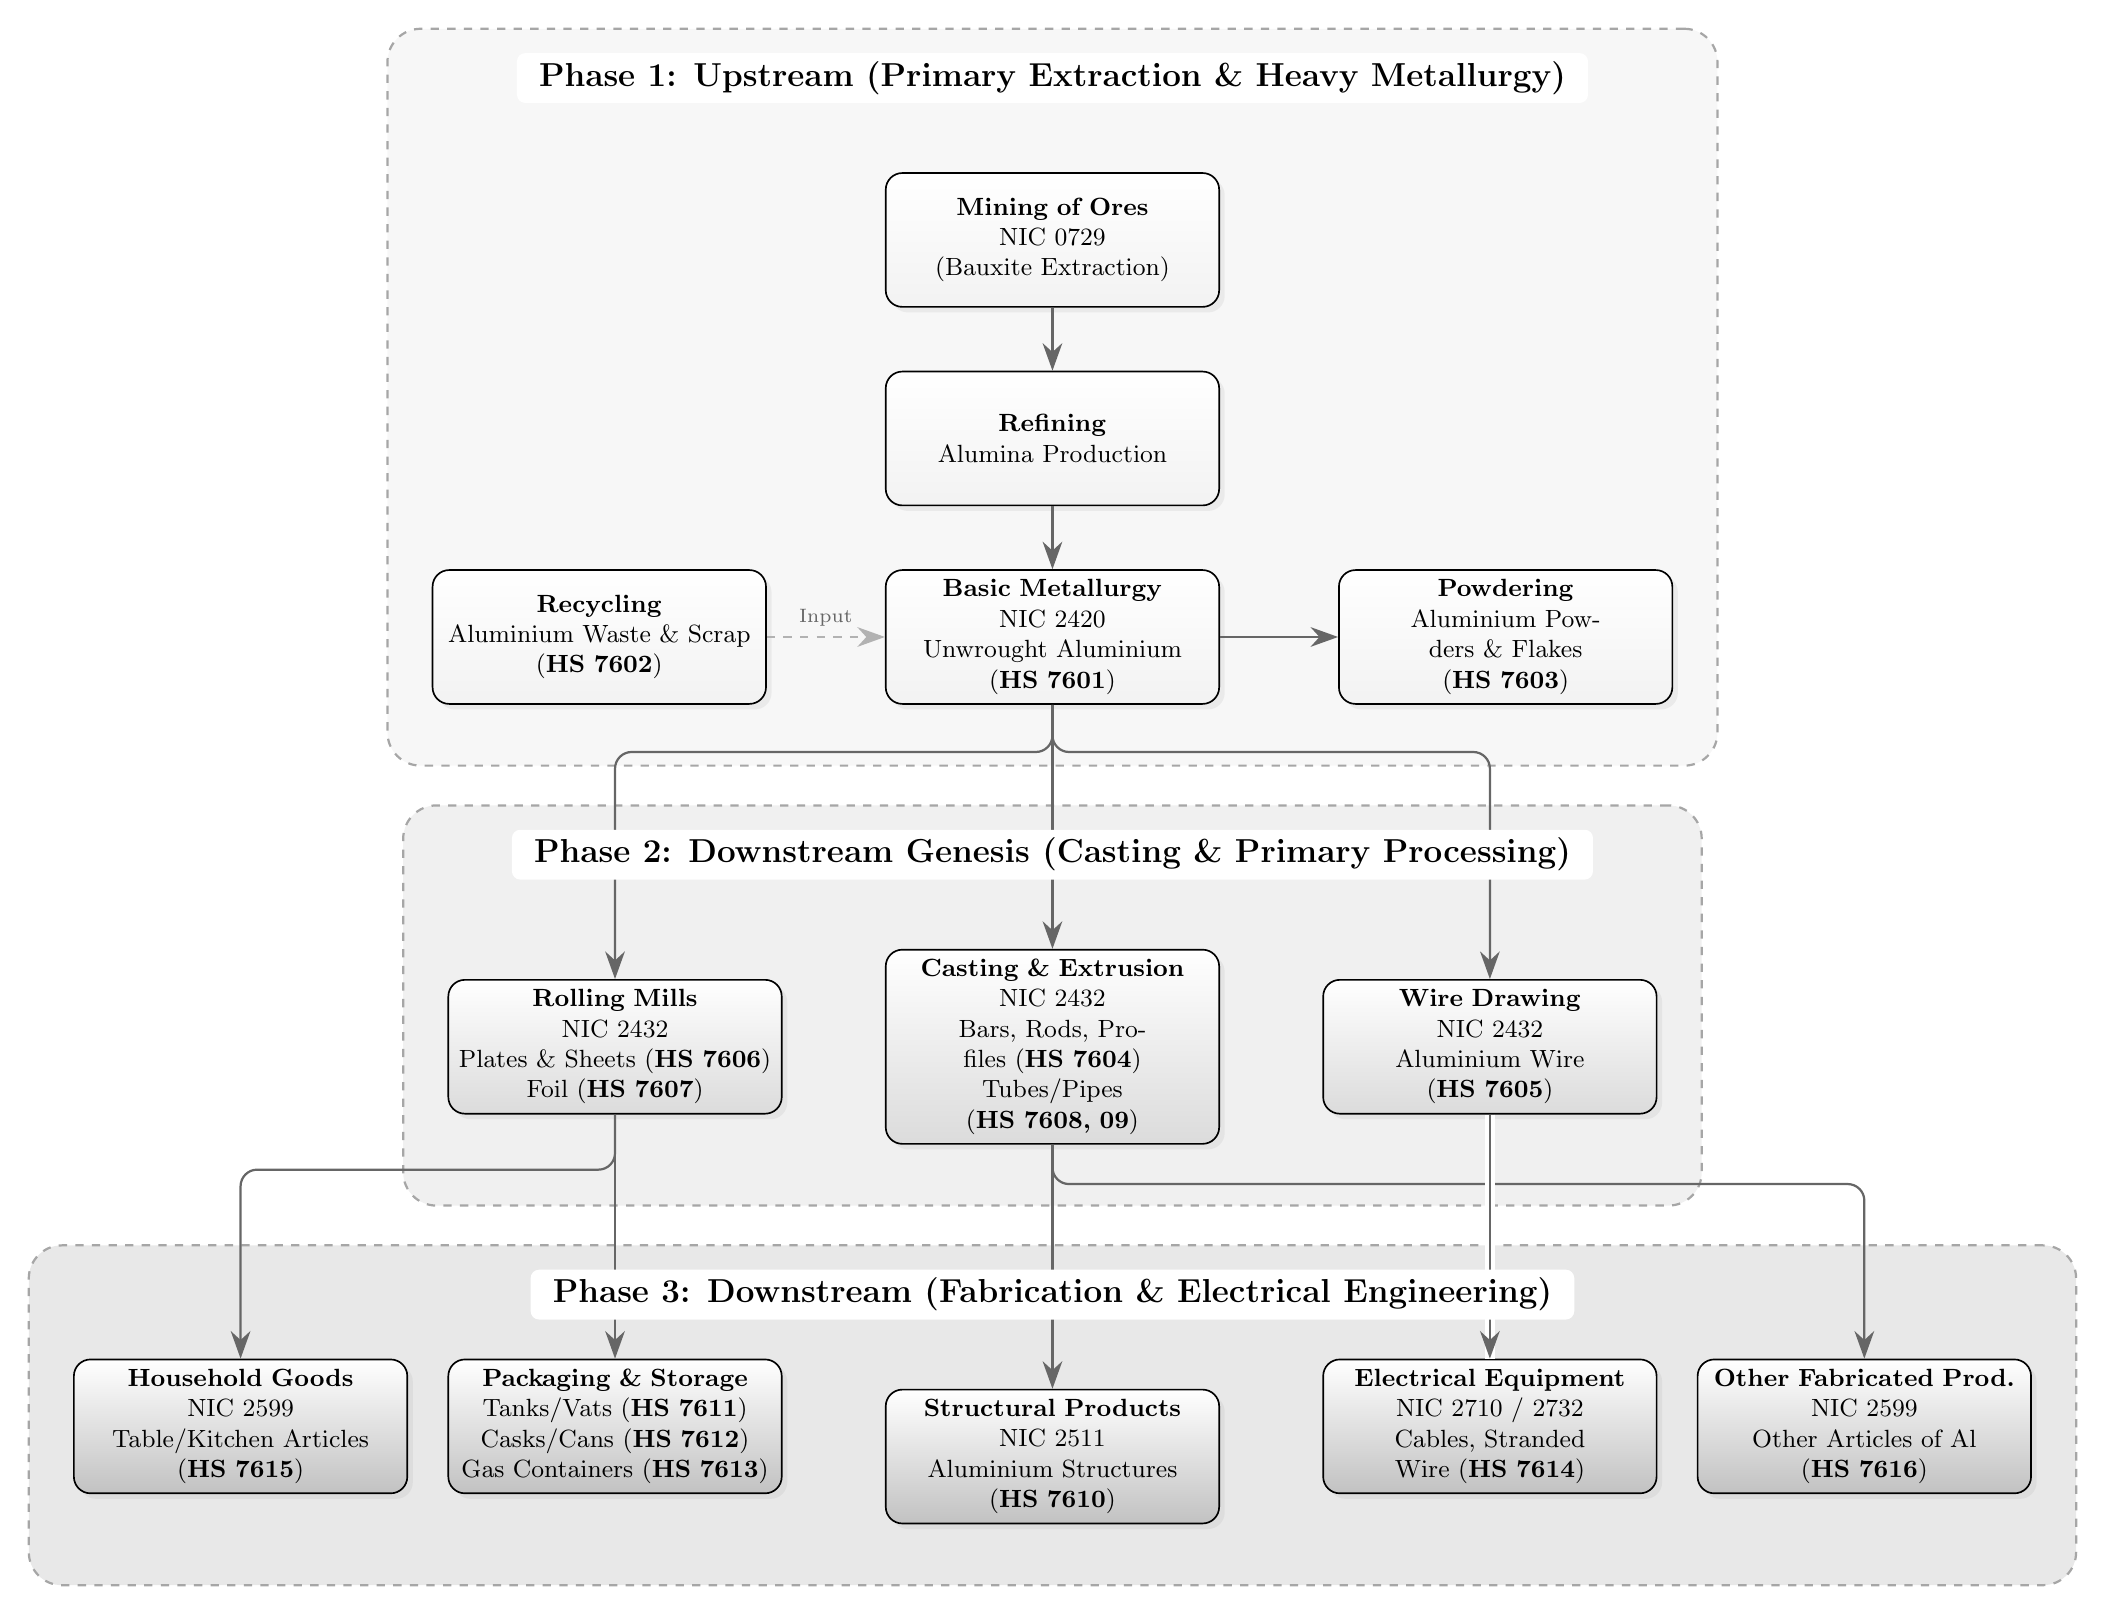
\begin{tikzpicture}[
        node distance=1.5cm and 1.3cm,
        box/.style={rectangle, draw, rounded corners=6pt, align=center, text width=4.0cm, minimum height=1.7cm, thick, font=\small, drop shadow={opacity=0.1, shadow xshift=2pt, shadow yshift=-2pt}},
        up/.style={box, top color=white, bottom color=g1, draw=black, line width=0.6pt},
        mid/.style={box, top color=white, bottom color=g2, draw=black, line width=0.6pt},
        down/.style={box, top color=white, bottom color=g3, draw=black, line width=0.6pt},
        arrow/.style={-{Stealth[length=3.5mm, width=2.5mm]}, thick, draw=gray!80!black, rounded corners=6pt},
        backarrow/.style={dashed, -{Stealth[length=3.5mm, width=2.5mm]}, thick, draw=gray!60, rounded corners=6pt},
        groupbox/.style={rectangle, rounded corners=12pt, draw=black!35, dashed, thick, inner xsep=16pt, inner ysep=22pt}
    ]
        % UPSTREAM PHASE
        \node[up] (unwrought) {\textbf{Basic Metallurgy} \\ NIC 2420 \\ Unwrought Aluminium \\ (\textbf{HS 7601})};
        \node[up] (alumina) [above=0.8cm of unwrought] {\textbf{Refining} \\ Alumina Production};
        \node[up] (bauxite) [above=0.8cm of alumina] {\textbf{Mining of Ores} \\ NIC 0729 \\ (Bauxite Extraction)};
        \node[up] (scrap) [left=1.5cm of unwrought] {\textbf{Recycling} \\ Aluminium Waste \& Scrap \\ (\textbf{HS 7602})};
        \node[up] (powder) [right=1.5cm of unwrought] {\textbf{Powdering} \\ Aluminium Powders \& Flakes \\ (\textbf{HS 7603})};

        % MIDSTREAM PHASE
        \node[mid] (extrusion) [below=3.1cm of unwrought] {\textbf{Casting \& Extrusion} \\ NIC 2432 \\ Bars, Rods, Profiles (\textbf{HS 7604}) \\ Tubes/Pipes (\textbf{HS 7608, 09})};
        \node[mid] (rolling) [left=1.3cm of extrusion] {\textbf{Rolling Mills} \\ NIC 2432 \\ Plates \& Sheets (\textbf{HS 7606}) \\ Foil (\textbf{HS 7607})};
        \node[mid] (drawing) [right=1.3cm of extrusion] {\textbf{Wire Drawing} \\ NIC 2432 \\ Aluminium Wire \\ (\textbf{HS 7605})};

        % DOWNSTREAM PHASE
        \node[down] (structures) [below=3.1cm of extrusion] {\textbf{Structural Products} \\ NIC 2511 \\ Aluminium Structures \\ (\textbf{HS 7610})};
        \node[down] (containers) [below=3.1cm of rolling] {\textbf{Packaging \& Storage} \\ Tanks/Vats (\textbf{HS 7611}) \\ Casks/Cans (\textbf{HS 7612}) \\ Gas Containers (\textbf{HS 7613})};
        \node[down] (household) [left=0.5cm of containers] {\textbf{Household Goods} \\ NIC 2599 \\ Table/Kitchen Articles \\ (\textbf{HS 7615})};
        \node[down] (cables) [below=3.1cm of drawing] {\textbf{Electrical Equipment} \\ NIC 2710 / 2732 \\ Cables, Stranded Wire (\textbf{HS 7614})};
        \node[down] (other) [right=0.5cm of cables] {\textbf{Other Fabricated Prod.} \\ NIC 2599 \\ Other Articles of Al \\ (\textbf{HS 7616})};

        % BACKGROUND GROUPING & LABELS
        \node (up_dummy) [above=0.8cm of bauxite] {};
        \node (mid_dummy) [above=0.8cm of extrusion] {};
        \node (down_dummy) [above=0.8cm of structures] {};
        \begin{scope}[on background layer]
            \node[groupbox, fill=black!3, fit=(up_dummy) (bauxite) (alumina) (unwrought) (scrap) (powder)] (up_group) {};
            \node[groupbox, fill=black!6, fit=(mid_dummy) (rolling) (extrusion) (drawing)] (mid_group) {};
            \node[groupbox, fill=black!9, fit=(down_dummy) (household) (containers) (structures) (cables) (other)] (down_group) {};
        \end{scope}


        % ARROWS
        \draw[arrow] (bauxite) -- (alumina);
        \draw[arrow] (alumina) -- (unwrought);
        \draw[backarrow] (scrap) -- node[above, font=\scriptsize, color=gray!80!black] {Input} (unwrought);
        \draw[arrow] (unwrought) -- (powder);
        \draw[arrow] (unwrought.south) -- +(0,-0.6) -| (rolling.north);
        \draw[arrow] (unwrought.south) -- (extrusion.north);
        \draw[arrow] (unwrought.south) -- +(0,-0.6) -| (drawing.north);
        \draw[arrow] (rolling.south) -- (containers.north);
        \draw[arrow] (rolling.south) -- +(0,-0.7) -| (household.north);
        \draw[arrow] (extrusion.south) -- (structures.north);
        \draw[arrow] (extrusion.south) -- +(0,-0.5) -| (other.north);
        \draw[line width=3.5pt, white] (drawing.south) -- (cables.north);
        \draw[arrow] (drawing.south) -- (cables.north);

        % PHASE LABELS -- drawn last, with opaque fills, so no connector
        % line can run through the heading text
        \node[anchor=north, font=\large\bfseries, color=black, yshift=-9pt,
              fill=white, rounded corners=3pt, inner xsep=8pt, inner ysep=3pt]
              at (up_group.north) {Phase 1: Upstream (Primary Extraction \& Heavy Metallurgy)};
        \node[anchor=north, font=\large\bfseries, color=black, yshift=-9pt,
              fill=white, rounded corners=3pt, inner xsep=8pt, inner ysep=3pt]
              at (mid_group.north) {Phase 2: Downstream Genesis (Casting \& Primary Processing)};
        \node[anchor=north, font=\large\bfseries, color=black, yshift=-9pt,
              fill=white, rounded corners=3pt, inner xsep=8pt, inner ysep=3pt]
              at (down_group.north) {Phase 3: Downstream (Fabrication \& Electrical Engineering)};
    \end{tikzpicture}
    }
    \captionsetup{font=normalsize, justification=centering}
    \caption{The Aluminium Value Chain, tracking industrial operations and HS Code progression. (reproduced for reference)}
\end{figure}

\begin{figure}[H]
    \centering
    \captionsetup{font={color=black, normalsize}, justification=centering}
    \caption{Global Primary Aluminum Consumption and its Forecast (in million metric tons) (reproduced for reference)}
    \vspace{0.5cm}

    \resizebox{\textwidth}{!}{%
    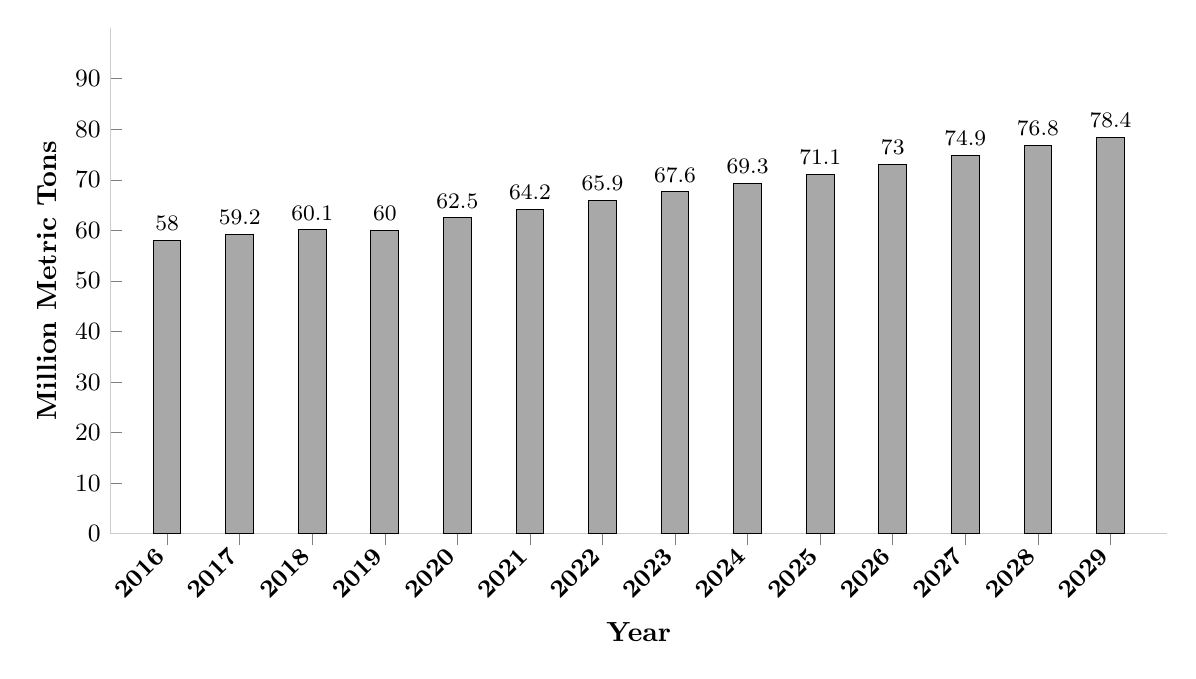
\begin{tikzpicture}
        \begin{axis}[
            ybar,
            width=15cm,
            height=8cm,
            bar width=10pt,
            ymin=0,
            ymax=100,
            ytick={0, 10, 20, 30, 40, 50, 60, 70, 80, 90},
            ylabel={\textbf{Million Metric Tons}},
            xlabel={\textbf{Year}},
            symbolic x coords={2016,2017,2018,2019,2020,2021,2022,2023,2024,2025,2026,2027,2028,2029},
            xtick=data,
            x tick label style={rotate=45, anchor=east, font=\small\bfseries},
            nodes near coords={\textbf{\pgfmathprintnumber\pgfplotspointmeta}},
            nodes near coords align={vertical},
            every node near coord/.append style={font=\footnotesize, color=black},
            tick label style={font=\small\bfseries},
            axis x line*=bottom,
            axis y line*=left,
            enlarge x limits=0.06,
            ymajorgrids=false,
            axis line style={gray!40},
            every axis plot post/.append style={fill=g4, draw=black, line width=0.35pt}
        ]
        \addplot coordinates {
            (2016, 58)
            (2017, 59.2)
            (2018, 60.1)
            (2019, 60)
            (2020, 62.5)
            (2021, 64.2)
            (2022, 65.9)
            (2023, 67.6)
            (2024, 69.3)
            (2025, 71.1)
            (2026, 73.0)
            (2027, 74.9)
            (2028, 76.8)
            (2029, 78.4)
        };
        \end{axis}
    \end{tikzpicture}%
    }

    \vspace{0.2cm}
    \raggedright
    Source: Statista
\end{figure}

\begin{figure}[H]
    \centering
    \captionsetup{font={color=black, normalsize}, justification=centering}
    \caption{Global Primary Aluminium Production by Region, 2011--2025 (thousand metric tonnes) (reproduced for reference)}

    \resizebox{\textwidth}{!}{%
    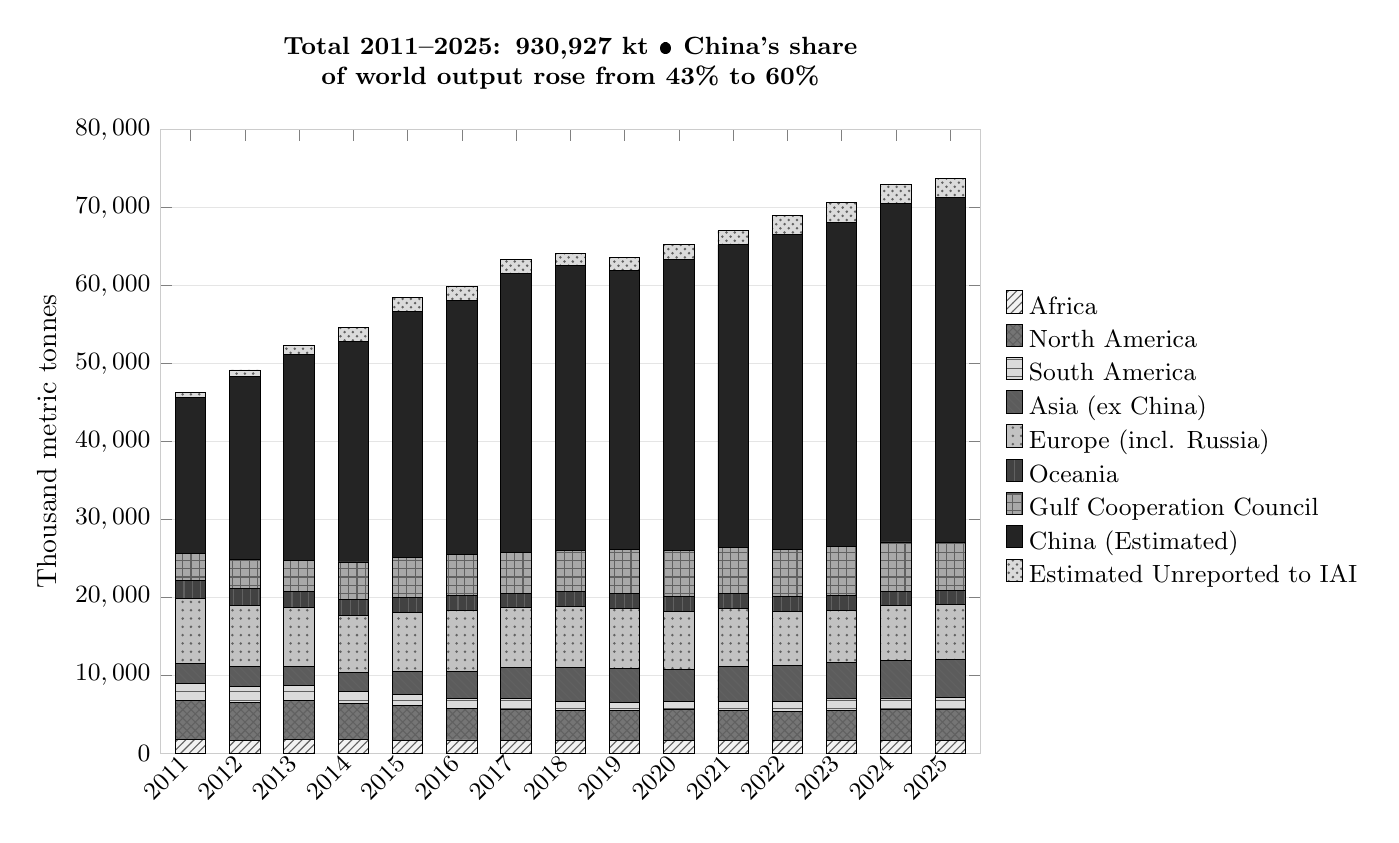
\begin{tikzpicture}
    \begin{axis}[
        ybar stacked,
        width=12cm,
        height=9.5cm,
        bar width=11pt,
        title={\textbf{Total 2011--2025: 930{,}927 kt \textbullet\ China's share of world output rose from 43\% to 60\%}},
        title style={yshift=5pt, font=\small\bfseries, align=center, text width=11cm},
        ylabel={Thousand metric tonnes},
        ymin=0, ymax=80000,
        ytick={0,10000,20000,30000,40000,50000,60000,70000,80000},
        scaled y ticks=false,
        yticklabel style={/pgf/number format/fixed, /pgf/number format/1000 sep={,}, font=\small},
        xtick={2011,2012,2013,2014,2015,2016,2017,2018,2019,2020,2021,2022,2023,2024,2025},
        x tick label style={/pgf/number format/1000 sep={}, rotate=45, anchor=east, font=\small},
        enlarge x limits=0.04,
        ymajorgrids=true,
        major grid style={gray!20},
        axis line style={gray!40},
        legend style={at={(1.02,0.5)}, anchor=west, legend columns=1, draw=none, font=\small},
        legend cell align={left},
    ]
    \addplot[fill=g1, draw=black, line width=0.35pt, postaction={pattern=north east lines, pattern color=black!62}] coordinates {(2011,1805) (2012,1639) (2013,1812) (2014,1746) (2015,1687) (2016,1691) (2017,1679) (2018,1668) (2019,1643) (2020,1605) (2021,1590) (2022,1620) (2023,1594) (2024,1576) (2025,1615)};
    \addlegendentry{Africa}

    \addplot[fill=g6, draw=black, line width=0.35pt, postaction={pattern=crosshatch, pattern color=black!62}] coordinates {(2011,4969) (2012,4851) (2013,4918) (2014,4585) (2015,4469) (2016,4027) (2017,3950) (2018,3774) (2019,3809) (2020,3976) (2021,3880) (2022,3743) (2023,3897) (2024,3983) (2025,3938)};
    \addlegendentry{North America}

    \addplot[fill=g2, draw=black, line width=0.35pt, postaction={pattern=horizontal lines, pattern color=black!62}] coordinates {(2011,2185) (2012,2052) (2013,1906) (2014,1543) (2015,1325) (2016,1361) (2017,1378) (2018,1164) (2019,1079) (2020,1006) (2021,1163) (2022,1288) (2023,1466) (2024,1521) (2025,1551)};
    \addlegendentry{South America}

    \addplot[fill=g7, draw=black, line width=0.35pt, postaction={pattern=north west lines, pattern color=black!62}] coordinates {(2011,2533) (2012,2535) (2013,2439) (2014,2429) (2015,3001) (2016,3442) (2017,3951) (2018,4415) (2019,4395) (2020,4140) (2021,4499) (2022,4591) (2023,4673) (2024,4812) (2025,4859)};
    \addlegendentry{Asia (ex China)}

    \addplot[fill=g3, draw=black, line width=0.35pt, postaction={pattern=dots, pattern color=black!62}] coordinates {(2011,8346) (2012,7928) (2013,7611) (2014,7360) (2015,7574) (2016,7760) (2017,7775) (2018,7782) (2019,7606) (2020,7487) (2021,7468) (2022,6994) (2023,6729) (2024,6996) (2025,7059)};
    \addlegendentry{Europe (incl. Russia)}

    \addplot[fill=g8, draw=black, line width=0.35pt, postaction={pattern=vertical lines, pattern color=black!62}] coordinates {(2011,2306) (2012,2186) (2013,2104) (2014,2035) (2015,1978) (2016,1971) (2017,1817) (2018,1917) (2019,1916) (2020,1912) (2021,1888) (2022,1843) (2023,1884) (2024,1863) (2025,1878)};
    \addlegendentry{Oceania}

    \addplot[fill=g4, draw=black, line width=0.35pt, postaction={pattern=grid, pattern color=black!62}] coordinates {(2011,3483) (2012,3662) (2013,3887) (2014,4832) (2015,5104) (2016,5197) (2017,5149) (2018,5331) (2019,5654) (2020,5833) (2021,5889) (2022,6074) (2023,6217) (2024,6346) (2025,6159)};
    \addlegendentry{Gulf Cooperation Council}

    \addplot[fill=g9, draw=black, line width=0.35pt] coordinates {(2011,20072) (2012,23534) (2013,26534) (2014,28317) (2015,31518) (2016,32641) (2017,35905) (2018,36485) (2019,35795) (2020,37337) (2021,38837) (2022,40430) (2023,41666) (2024,43396) (2025,44219)};
    \addlegendentry{China (Estimated)}

    \addplot[fill=g2, draw=black, line width=0.35pt, postaction={pattern=crosshatch dots, pattern color=black!62}] coordinates {(2011,576) (2012,780) (2013,1080) (2014,1800) (2015,1800) (2016,1800) (2017,1800) (2018,1630) (2019,1760) (2020,2029) (2021,1878) (2022,2455) (2023,2590) (2024,2516) (2025,2516)};
    \addlegendentry{Estimated Unreported to IAI}

    \end{axis}
    \end{tikzpicture}%
    }

    \vspace{0.2cm}
    \raggedright
    \small Source: International Aluminium Institute (IAI); annual totals of monthly reported primary aluminium production. Data for Jan--May 2026 are available but omitted for year-on-year comparability. From 2020 onward the IAI reports European output on a combined ``Europe (incl.\ Russia)'' basis; earlier ``Western \& Central'' and ``Russia \& Eastern'' figures are aggregated here for a consistent series.
\end{figure}

\begin{figure}[H]
    \centering
    \captionsetup{font={color=black, normalsize}, justification=centering}
    \caption{Top Exporting Countries of Primary Aluminum to India in 2021 (Tons) (reproduced for reference)}
    \vspace{0.5cm}

    \resizebox{\textwidth}{!}{%
    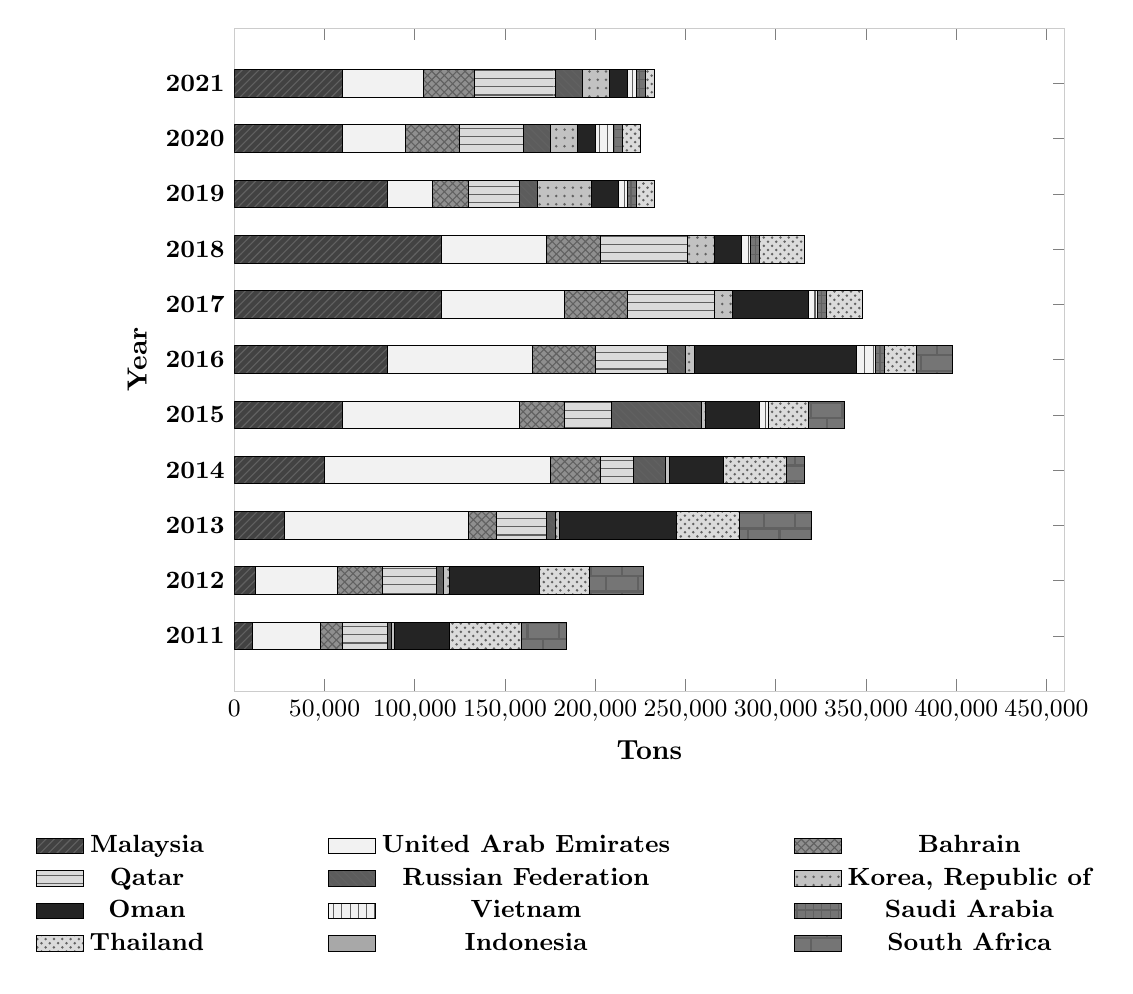
\begin{tikzpicture}
        \begin{axis}[
            xbar stacked,
            width=\textwidth,
            height=10cm,
            bar width=10pt,
            xmin=0,
            xmax=460000,
            xtick={0, 50000, 100000, 150000, 200000, 250000, 300000, 350000, 400000, 450000},
            scaled x ticks=false,
            xticklabel style={/pgf/number format/fixed, font=\small\bfseries},
            xlabel={\textbf{Tons}},
            ylabel={\textbf{Year}},
            yticklabel style={font=\small\bfseries},
            symbolic y coords={2011,2012,2013,2014,2015,2016,2017,2018,2019,2020,2021},
            ytick=data,
            axis line style={gray!40},
            legend style={
                at={(0.4,-0.2)},
                anchor=north,
                legend columns=3,
                draw=none,
                font=\small\bfseries,
                /tikz/every even column/.append style={column sep=1.5cm}
            },
            area legend
        ]

        \addplot[fill=g8, draw=black, line width=0.35pt, postaction={pattern=north east lines, pattern color=black!62}] coordinates {(10000,2011) (12000,2012) (28000,2013) (50000,2014) (60000,2015) (85000,2016) (115000,2017) (115000,2018) (85000,2019) (60000,2020) (60000,2021)};
        \addlegendentry{Malaysia}

        \addplot[fill=g1, draw=black, line width=0.35pt] coordinates {(38000,2011) (45000,2012) (102000,2013) (125000,2014) (98000,2015) (80000,2016) (68000,2017) (58000,2018) (25000,2019) (35000,2020) (45000,2021)};
        \addlegendentry{United Arab Emirates}

        \addplot[fill=g5, draw=black, line width=0.35pt, postaction={pattern=crosshatch, pattern color=black!62}] coordinates {(12000,2011) (25000,2012) (15000,2013) (28000,2014) (25000,2015) (35000,2016) (35000,2017) (30000,2018) (20000,2019) (30000,2020) (28000,2021)};
        \addlegendentry{Bahrain}

        \addplot[fill=g2, draw=black, line width=0.35pt, postaction={pattern=horizontal lines, pattern color=black!62}] coordinates {(25000,2011) (30000,2012) (28000,2013) (18000,2014) (26000,2015) (40000,2016) (48000,2017) (48000,2018) (28000,2019) (35000,2020) (45000,2021)};
        \addlegendentry{Qatar}

        \addplot[fill=g7, draw=black, line width=0.35pt, postaction={pattern=north west lines, pattern color=black!62}] coordinates {(2000,2011) (4000,2012) (5000,2013) (18000,2014) (50000,2015) (10000,2016) (0,2017) (0,2018) (10000,2019) (15000,2020) (15000,2021)};
        \addlegendentry{Russian Federation}

        \addplot[fill=g3, draw=black, line width=0.35pt, postaction={pattern=dots, pattern color=black!62}] coordinates {(2000,2011) (3000,2012) (2000,2013) (2000,2014) (2000,2015) (5000,2016) (10000,2017) (15000,2018) (30000,2019) (15000,2020) (15000,2021)};
        \addlegendentry{Korea, Republic of}

        \addplot[fill=g9, draw=black, line width=0.35pt] coordinates {(30000,2011) (50000,2012) (65000,2013) (30000,2014) (30000,2015) (90000,2016) (42000,2017) (15000,2018) (15000,2019) (10000,2020) (10000,2021)};
        \addlegendentry{Oman}

        \addplot[fill=g1, draw=black, line width=0.35pt, postaction={pattern=vertical lines, pattern color=black!62}] coordinates {(0,2011) (0,2012) (0,2013) (0,2014) (5000,2015) (10000,2016) (5000,2017) (5000,2018) (5000,2019) (10000,2020) (5000,2021)};
        \addlegendentry{Vietnam}

        \addplot[fill=g6, draw=black, line width=0.35pt, postaction={pattern=grid, pattern color=black!62}] coordinates {(0,2011) (0,2012) (0,2013) (0,2014) (0,2015) (5000,2016) (5000,2017) (5000,2018) (5000,2019) (5000,2020) (5000,2021)};
        \addlegendentry{Saudi Arabia}

        \addplot[fill=g2, draw=black, line width=0.35pt, postaction={pattern=crosshatch dots, pattern color=black!62}] coordinates {(40000,2011) (28000,2012) (35000,2013) (35000,2014) (22000,2015) (18000,2016) (20000,2017) (25000,2018) (10000,2019) (10000,2020) (5000,2021)};
        \addlegendentry{Thailand}

        \addplot[fill=g4, draw=black, line width=0.35pt] coordinates {(0,2011) (0,2012) (0,2013) (0,2014) (0,2015) (0,2016) (0,2017) (0,2018) (0,2019) (0,2020) (0,2021)};
        \addlegendentry{Indonesia}

        \addplot[fill=g6, draw=black, line width=0.35pt, postaction={pattern=bricks, pattern color=black!62}] coordinates {(25000,2011) (30000,2012) (40000,2013) (10000,2014) (20000,2015) (20000,2016) (0,2017) (0,2018) (0,2019) (0,2020) (0,2021)};
        \addlegendentry{South Africa}

        \end{axis}
    \end{tikzpicture}%
    }

    \vspace{1.5cm}
    \raggedright
    Source: ITC Trade Map
\end{figure}

\begin{figure}[H]
    \centering
    \captionsetup{font={color=black, normalsize}, justification=centering}
    \caption{Average Effective Rate of Protection by partner and period (reproduced for reference)}
    \vspace{0.3cm}

    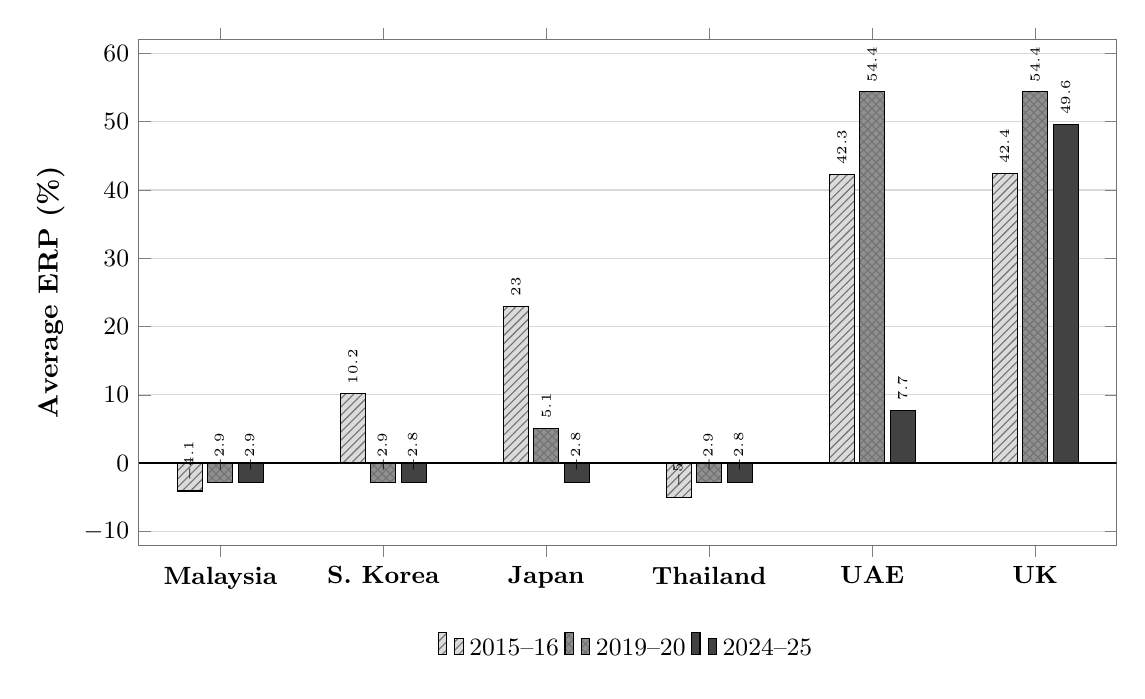
\begin{tikzpicture}
    \begin{axis}[
        ybar,
        width=14cm, height=8cm,
        bar width=9pt,
        ymin=-12, ymax=62,
        ytick={-10,0,10,20,30,40,50,60},
        ylabel={\textbf{Average ERP (\%)}},
        symbolic x coords={Malaysia,{S. Korea},Japan,Thailand,UAE,UK},
        xtick=data,
        x tick label style={font=\small\bfseries},
        tick label style={font=\small},
        ymajorgrids=true, major grid style={black!15},
        axis line style={black!55},
        legend style={at={(0.5,-0.16)}, anchor=north, legend columns=3, draw=none, font=\small},
        legend cell align={left},
        nodes near coords={\pgfmathprintnumber[fixed, precision=1]\pgfplotspointmeta},
        every node near coord/.append style={font=\tiny, rotate=90, anchor=west},
    ]
    \addplot[fill=g2, draw=black, line width=0.4pt, postaction={pattern=north east lines, pattern color=black!55}]
      coordinates {(Malaysia,-4.08) ({S. Korea},10.15) (Japan,23.00) (Thailand,-5.00) (UAE,42.31) (UK,42.38)};
    \addlegendentry{2015--16}
    \addplot[fill=g5, draw=black, line width=0.4pt, postaction={pattern=crosshatch, pattern color=black!55}]
      coordinates {(Malaysia,-2.85) ({S. Korea},-2.85) (Japan,5.08) (Thailand,-2.85) (UAE,54.38) (UK,54.38)};
    \addlegendentry{2019--20}
    \addplot[fill=g8, draw=black, line width=0.4pt]
      coordinates {(Malaysia,-2.85) ({S. Korea},-2.81) (Japan,-2.81) (Thailand,-2.81) (UAE,7.69) (UK,49.62)};
    \addlegendentry{2024--25}
    \draw[black, thick] ({rel axis cs:0,0}|-{axis cs:Malaysia,0}) -- ({rel axis cs:1,0}|-{axis cs:Malaysia,0});
    \end{axis}
    \end{tikzpicture}

    \vspace{0.2cm}
    \raggedright
    \small Source: Our estimates from MOSPI Supply Use Tables and partner tariff schedules. Bars below the zero line denote negative effective protection. The UK series is a non-preferential (MFN) benchmark.
\end{figure}

\begin{figure}[H]
    \centering
    \captionsetup{font={color=black, normalsize}, justification=centering}
    \caption{Gross Value Added and Persons Engaged, index 2011--12 $=$ 100 (reproduced for reference)}
    \vspace{0.3cm}

    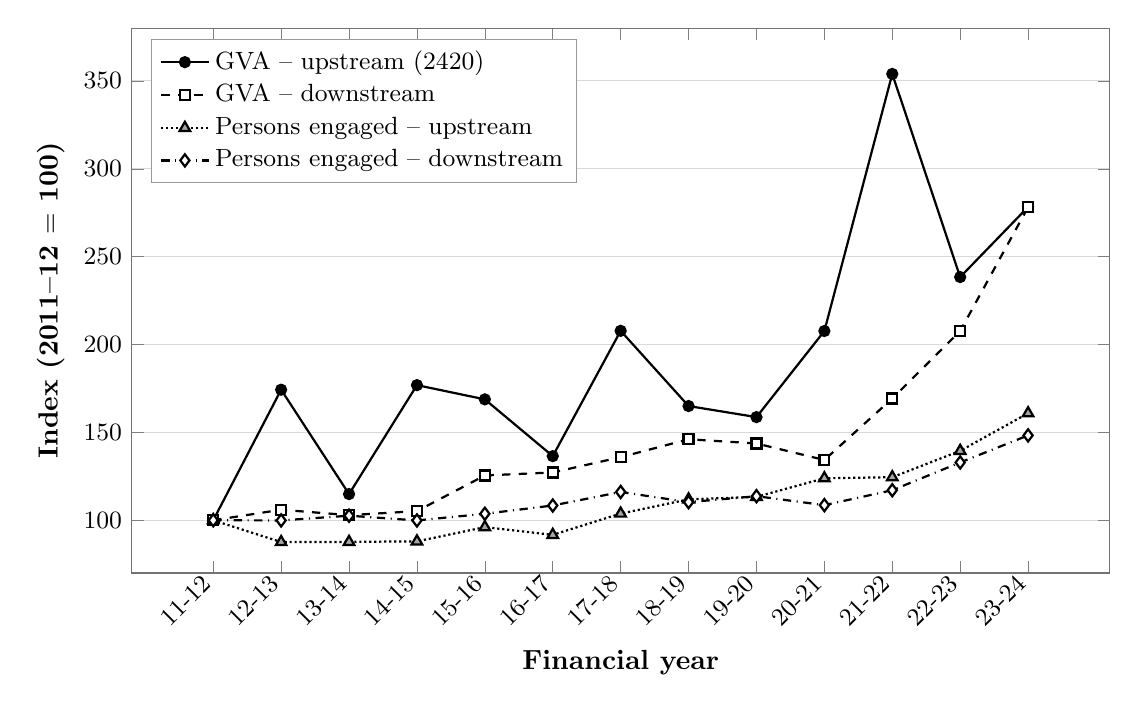
\begin{tikzpicture}
    \begin{axis}[
        width=14cm, height=8.5cm,
        ymin=70, ymax=380,
        ylabel={\textbf{Index (2011--12 $=$ 100)}},
        xlabel={\textbf{Financial year}},
        symbolic x coords={11-12,12-13,13-14,14-15,15-16,16-17,17-18,18-19,19-20,20-21,21-22,22-23,23-24},
        xtick=data,
        x tick label style={rotate=45, anchor=east, font=\small},
        tick label style={font=\small},
        ymajorgrids=true, major grid style={black!15},
        axis line style={black!55},
        legend style={at={(0.02,0.98)}, anchor=north west, draw=black!40, fill=white, font=\small},
        legend cell align={left},
        cycle list name=black white,
    ]
    \addplot[black, thick, mark=*, mark size=1.8pt] coordinates {(11-12,100.0)(12-13,174.3)(13-14,114.9)(14-15,176.9)(15-16,168.8)(16-17,136.5)(17-18,207.8)(18-19,165.0)(19-20,158.7)(20-21,207.7)(21-22,354.0)(22-23,238.4)(23-24,278.3)};
    \addlegendentry{GVA -- upstream (2420)}
    \addplot[black, thick, dashed, mark=square*, mark size=1.8pt, mark options={solid, fill=white}] coordinates {(11-12,100.0)(12-13,106.0)(13-14,102.9)(14-15,105.2)(15-16,125.5)(16-17,127.2)(17-18,135.9)(18-19,146.1)(19-20,143.7)(20-21,134.3)(21-22,169.3)(22-23,207.7)(23-24,278.2)};
    \addlegendentry{GVA -- downstream}
    \addplot[black, densely dotted, thick, mark=triangle*, mark size=2.2pt, mark options={solid, fill=black!35}] coordinates {(11-12,100.0)(12-13,87.6)(13-14,87.7)(14-15,88.0)(15-16,96.1)(16-17,91.7)(17-18,103.8)(18-19,111.9)(19-20,113.3)(20-21,123.9)(21-22,124.5)(22-23,139.5)(23-24,160.9)};
    \addlegendentry{Persons engaged -- upstream}
    \addplot[black, dashdotted, thick, mark=diamond*, mark size=2.2pt, mark options={solid, fill=white}] coordinates {(11-12,100.0)(12-13,99.9)(13-14,102.6)(14-15,99.9)(15-16,103.7)(16-17,108.4)(17-18,116.1)(18-19,110.3)(19-20,113.7)(20-21,108.6)(21-22,117.1)(22-23,132.9)(23-24,148.3)};
    \addlegendentry{Persons engaged -- downstream}
    \end{axis}
    \end{tikzpicture}

    \vspace{0.2cm}
    \raggedright
    \small Source: Our calculations from ASI All-India summary results. GVA at current prices (nominal; no deflator applied). Upstream $=$ NIC~2420; downstream $=$ NIC~2432, 2511, 2599, 2710, 2732, 3030.
\end{figure}

\begin{figure}[H]
    \centering
    \captionsetup{font={color=black, normalsize}, justification=centering}
    \caption{Gross Value Added per person engaged (INR lakh, current prices) (reproduced for reference)}
    \vspace{0.3cm}

    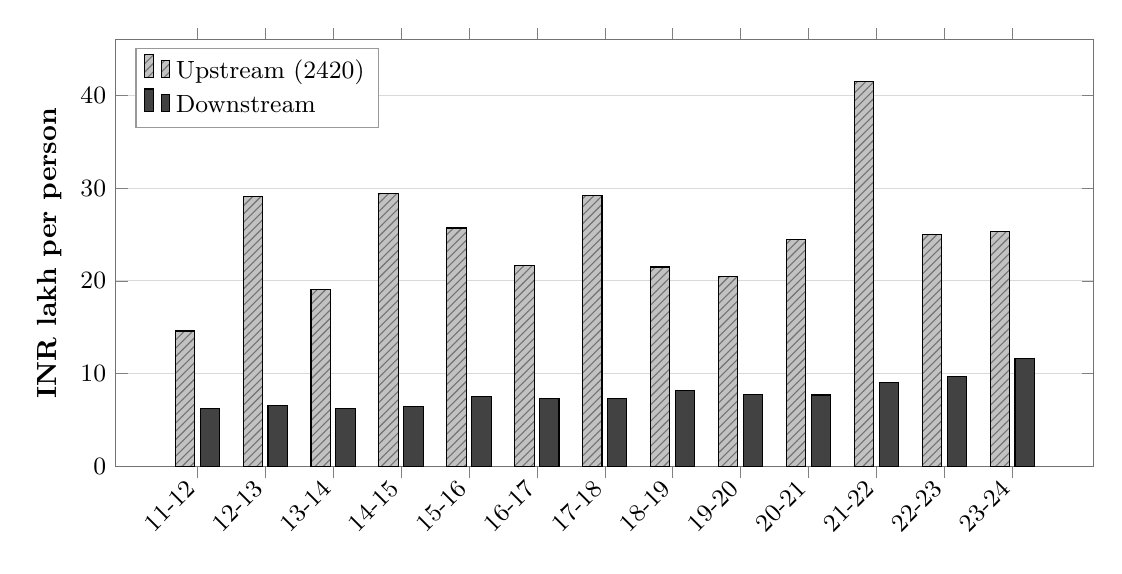
\begin{tikzpicture}
    \begin{axis}[
        ybar,
        width=14cm, height=7cm,
        bar width=7pt,
        ymin=0, ymax=46,
        ylabel={\textbf{INR lakh per person}},
        symbolic x coords={11-12,12-13,13-14,14-15,15-16,16-17,17-18,18-19,19-20,20-21,21-22,22-23,23-24},
        xtick=data,
        x tick label style={rotate=45, anchor=east, font=\small},
        tick label style={font=\small},
        ymajorgrids=true, major grid style={black!15},
        axis line style={black!55},
        legend style={at={(0.02,0.98)}, anchor=north west, draw=black!40, fill=white, font=\small},
        legend cell align={left},
    ]
    \addplot[fill=g3, draw=black, line width=0.4pt, postaction={pattern=north east lines, pattern color=black!55}]
      coordinates {(11-12,14.6)(12-13,29.1)(13-14,19.1)(14-15,29.4)(15-16,25.7)(16-17,21.7)(17-18,29.2)(18-19,21.5)(19-20,20.5)(20-21,24.5)(21-22,41.5)(22-23,25.0)(23-24,25.3)};
    \addlegendentry{Upstream (2420)}
    \addplot[fill=g8, draw=black, line width=0.4pt]
      coordinates {(11-12,6.2)(12-13,6.6)(13-14,6.2)(14-15,6.5)(15-16,7.5)(16-17,7.3)(17-18,7.3)(18-19,8.2)(19-20,7.8)(20-21,7.7)(21-22,9.0)(22-23,9.7)(23-24,11.6)};
    \addlegendentry{Downstream}
    \end{axis}
    \end{tikzpicture}

    \vspace{0.2cm}
    \raggedright
    \small Source: Our calculations from ASI All-India summary results. A \emph{lower} bar denotes greater labour intensity---more persons engaged per unit of value added.
\end{figure}

\begin{figure}[H]
    \centering
    \captionsetup{font={color=black, normalsize}, justification=centering}
    \caption{Workers employed through contractors as a share of total workers (per cent) (reproduced for reference)}
    \vspace{0.3cm}

    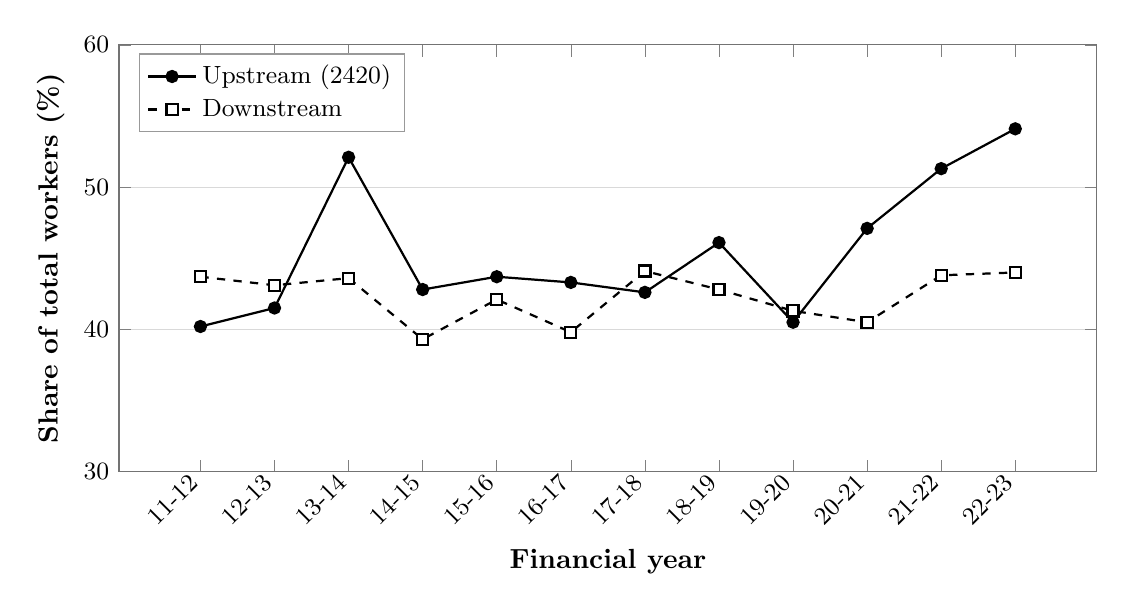
\begin{tikzpicture}
    \begin{axis}[
        width=14cm, height=7cm,
        ymin=30, ymax=60,
        ylabel={\textbf{Share of total workers (\%)}},
        xlabel={\textbf{Financial year}},
        symbolic x coords={11-12,12-13,13-14,14-15,15-16,16-17,17-18,18-19,19-20,20-21,21-22,22-23},
        xtick=data,
        x tick label style={rotate=45, anchor=east, font=\small},
        tick label style={font=\small},
        ymajorgrids=true, major grid style={black!15},
        axis line style={black!55},
        legend style={at={(0.02,0.98)}, anchor=north west, draw=black!40, fill=white, font=\small},
        legend cell align={left},
    ]
    \addplot[black, thick, mark=*, mark size=2pt] coordinates {(11-12,40.2)(12-13,41.5)(13-14,52.1)(14-15,42.8)(15-16,43.7)(16-17,43.3)(17-18,42.6)(18-19,46.1)(19-20,40.5)(20-21,47.1)(21-22,51.3)(22-23,54.1)};
    \addlegendentry{Upstream (2420)}
    \addplot[black, thick, dashed, mark=square*, mark size=2pt, mark options={solid, fill=white}] coordinates {(11-12,43.7)(12-13,43.1)(13-14,43.6)(14-15,39.3)(15-16,42.1)(16-17,39.8)(17-18,44.1)(18-19,42.8)(19-20,41.3)(20-21,40.5)(21-22,43.8)(22-23,44.0)};
    \addlegendentry{Downstream}
    \end{axis}
    \end{tikzpicture}

    \vspace{0.2cm}
    \raggedright
    \small Source: Our calculations from ASI All-India summary results. \textbf{2023--24 is omitted:} in that year the published directly-employed and contract-worker counts do not sum to total workers (an aggregate residual of 193,626 workers across the eight classes examined), whereas the identity holds exactly in every year from 2011--12 to 2022--23. The series is therefore truncated rather than presented on an inconsistent basis.
\end{figure}

\begin{figure}[H]
    \centering
    \captionsetup{font={color=black, normalsize}, justification=centering}
    \caption{Estimated corporate tax contribution (INR thousand crore) (reproduced for reference)}
    \vspace{0.3cm}

    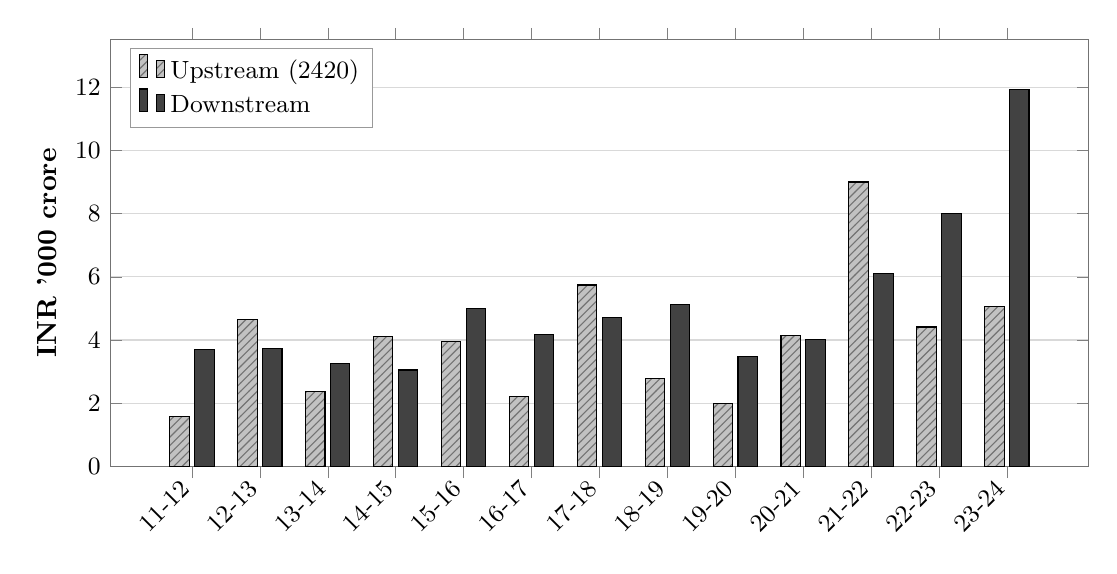
\begin{tikzpicture}
    \begin{axis}[
        ybar,
        width=14cm, height=7cm,
        bar width=7pt,
        ymin=0, ymax=13.5,
        ylabel={\textbf{INR '000 crore}},
        symbolic x coords={11-12,12-13,13-14,14-15,15-16,16-17,17-18,18-19,19-20,20-21,21-22,22-23,23-24},
        xtick=data,
        x tick label style={rotate=45, anchor=east, font=\small},
        tick label style={font=\small},
        ymajorgrids=true, major grid style={black!15},
        axis line style={black!55},
        legend style={at={(0.02,0.98)}, anchor=north west, draw=black!40, fill=white, font=\small},
        legend cell align={left},
    ]
    \addplot[fill=g3, draw=black, line width=0.4pt, postaction={pattern=north east lines, pattern color=black!55}]
      coordinates {(11-12,1.57)(12-13,4.64)(13-14,2.38)(14-15,4.10)(15-16,3.94)(16-17,2.22)(17-18,5.74)(18-19,2.78)(19-20,1.99)(20-21,4.13)(21-22,9.00)(22-23,4.41)(23-24,5.06)};
    \addlegendentry{Upstream (2420)}
    \addplot[fill=g8, draw=black, line width=0.4pt]
      coordinates {(11-12,3.69)(12-13,3.72)(13-14,3.25)(14-15,3.05)(15-16,4.99)(16-17,4.18)(17-18,4.72)(18-19,5.12)(19-20,3.49)(20-21,4.01)(21-22,6.09)(22-23,7.99)(23-24,11.94)};
    \addlegendentry{Downstream}
    \end{axis}
    \end{tikzpicture}

    \vspace{0.2cm}
    \raggedright
    \small Source: Our calculations from ASI All-India summary results. Corporate tax estimated as net profit $\times$ the effective corporate tax rate for each year; loss-making observations excluded rather than netted (see Section~\ref{sec:asi_method}).
\end{figure}

\end{document}
